\documentclass[polish,12pt]{article} 
\usepackage{times}
\usepackage{graphicx} % Required for inserting images
\usepackage[a4paper,twoside,left=2.0cm,right=1.5cm,top=1.5cm,bottom=1.5cm]{geometry}
\usepackage{indentfirst}%wciecia a nowych akapitach
\usepackage[T1]{fontenc}
\usepackage[utf8]{inputenc}
\usepackage[polish]{babel}
\usepackage[hidelinks]{hyperref}
\usepackage[dvipsnames]{xcolor}
\usepackage{subfigure}
\usepackage{float}

\usepackage[section]{placeins}

\usepackage{setspace}


%definicja przydatnych poleceń
\newcommand{\kierunek}{Kierunek: INFORMATYKA}
\newcommand{\specjalnosc}{Specjalność: Programowanie}
\newcommand{\autor}{Oleksandr Lobchenko}
\newcommand{\album}{w68317}
\newcommand{\temat}{APLIKACJA DESKTOPOWA "SZPITAL+"}
%\newcommand{\typpracy}{PRACA DYPLOMOWA INŻYNIERSKA}
\newcommand{\miasto}{Rzeszów}
\newcommand{\rok}{2024}

\usepackage{tocloft} % dla zmiany spisu treści
\renewcommand{\contentsname}{\HUGE}
\renewcommand\cftsecfont{\LARGE\textbf}
\renewcommand\cftsubsecpagefont{\large}

\begin{document}


% *************** Strona tytułowa ***************
% *************** Strony tytułowe ***************

% ************************************************************
% W tym miejscu znajduje sie definicja wyglądu pierwszych stron:
% strony tytułowej, strony z oświadczeniem o treści pracy
% i strony ze spisem treści
% ************************************************************
% *************** Strona tytułowa ***************
%umieszczenie logo i nazwy uczelni
\noindent
\parbox{65mm}{
\includegraphics[width=13.0cm, height=3.0cm]{logoWSIiZ}}

\vspace{10mm}
\begin{center}
{\Large{}\textbf{\wydzial}}
\end{center}
\vspace{10mm}
\noindent
\hspace{30mm}{\Large{}\textbf{\kierunek}}\\

\noindent
\hspace{30mm}{\Large{}\textbf{\specjalnosc}}
\vspace{30mm}
\begin{center}
	{\large{}\autor}\\
	{\large{}\album}\\
	\vspace{15pt}
	{\huge{}\textbf{\textit{\temat}}}\\
        \vspace{20pt}
	{\normalsize{}Prowadzący: \prowadzacy}\\
	\vspace{100pt}
	{\LARGE{}\textbf{\typpracy}}\\
	\vspace{190pt}
	{\large{}\textbf{\miasto {} \rok}}
\end{center}

% pusta zawartość stopki - brak numeru strony
\thispagestyle{empty}

% *************** Strona z oświadczeniem o treści pracy ***************
\newpage
\text{}

\thispagestyle{empty}
\newpage


% *************** Spis treści ***************
\tableofcontents
% pusta zawartość stopki - brak numeru strony
\thispagestyle{empty}
\newpage

% *************** Koniec pliku front.tex ***************


% *************** Wstęp ***************
\chapter*{Wstęp}

\textquotedbl Aplikacja desktopowa Szpital+\textquotedbl{} jest aplikacją mającą na celu zmodernizowanie i usprawnienie codziennych operacji w placówkach medycznych. Jest to program umożliwiający do przechowywania i dodawania informacji dotyczących szpitalu. Medycyna zajmuje bardzo ważną część naszego życia. Dlatego uważam, że ułatwienie komunikacji między pracownikami zaoszczędzi czas i ulepszy jakość pracy.

% *************** Cele ***************
\begin{flushleft}
\section{\LARGE{Założenia/Cele projektu}}
\end{flushleft}

\begin{flushleft}
\large{\hspace{5mm}Celem głównym projektu jest stworzenie kompleksowej aplikacji desktopowej, mającej na celu usprawnienie procesów zarządzania w środowisku szpitalnym. Aplikacja \textquotedbl Szpital+\textquotedbl{} ma usprawnić gromadzenie danych medycznych oraz zwiększyć efektywność komunikacji w placówce medycznej. Aplikacja posiada 4 klienta, funkcjonalność których się różni:}
\renewcommand{\labelenumi}{\alph{enumi})}
\begin{enumerate}
    \item{Klient Głównego Kierownika (sekcja \ref{subsec:gl_kier})}
    \item{Klient Kierownika Działu (sekcja ~\ref{subsec:kier})} 
    \item{Klient Recepcjonisty (sekcja ~\ref{subsec:recep})}
    \item{Klient Lekarza (sekcja ~\ref{subsec:lekarz})}
\end{enumerate}
\end{flushleft}

% *************** Wymagania ***************
\begin{flushleft}
\section{\LARGE{Wymagania funkcjonalne}}
\end{flushleft}

\begin{flushleft}
    \subsection{\large{Ogólne funkcjonalności pracowników\label{subsec:gl_kier}}}
    \begin{itemize}
        \item{Przegląd informacji o siebie (sekcja ~\ref{subsec:przeg_inf})}
        \item{Wylogowanie się}
    \end{itemize}
\end{flushleft}

%\renewcommand{\labelitemi}{\textsc{-}}
\begin{flushleft}
    \subsection{\large{Klient Głównego Kierownika\label{subsec:gl_kier}}}
    \begin{itemize}
        \item{Wyświetlenie listy pracowników (sekcja ~\ref{subsec:wyst_prac})}
    \end{itemize}
\end{flushleft}

\begin{flushleft}
    \subsection{\large{Klient Kierownika Działu\label{subsec:kier}}}
    \begin{itemize}
        \item{Wyświetlenie listy lekarzy (sekcja ~\ref{subsec:wyst_lekrz})}
    \end{itemize}
\end{flushleft}

\begin{flushleft}
    \subsection{\large{Klient Recepcjonisty\label{subsec:recep}}}
    \begin{itemize}
        \item{Wyświetlenie listy lekarzy (sekcja ~\ref{subsec:wyst_lekrz})}
        \item{Funkcja dodawania pacjentów (sekcja ~\ref{subsec:dodn_pacjn})}
        % \item{Przegląd harmonogramu pacjenta (sekcja ~\ref{subsec:wyst_harm_klnt})}
        \item{Funkcja przeglądu wszystkich wizyt (sekcja ~\ref{subsec:przeg_wiz})}
    \end{itemize}
\end{flushleft}

\begin{flushleft}
    \subsection{\large{Klient Lekarza\label{subsec:lekarz}}}
    \begin{itemize}
        \item{Funkcja ustalenia swoich wizytów (sekcja ~\ref{subsec:ust_wiz})}
        \item{Przegląd swojego harmonogramu (sekcja ~\ref{subsec:wyst_harm_lekrz})}
        \item{Przegląd informacji o pacjencie (sekcja ~\ref{subsec:przeg_inf})}
        \item{Przegląd ksiązek lekarskich pacjentów (sekcja ~\ref{subsec:przeg_ks_lekr})}
    \end{itemize}
\end{flushleft}

\begin{flushleft}
    \subsection{\Large{Opis funkcjonalności}}
    \subsubsection{\large{Przegląd informacji}\label{subsec:przeg_inf}}
    Wyświetla informacje:
    \begin{itemize}
        \item{Dla pracownika: id pracownika, imię, nazwisko, dział szpitalu, specjalność, pesel, adres zamieszkania, datę urodzenia, miejscowość, numer telefonu, datę zatrudnienia, wynagrodzenie, email.}
        \item{Dla pacjenta: id pracjenta, imię, nazwisko, pesel, adres zamieszkania, datę urodzenia, miejscowość, numer telefonu}\label{item:info}
    \end{itemize}
\end{flushleft}

\begin{flushleft}
    \subsubsection{\large{Wyświetlenie listy pracowników}\label{subsec:wyst_prac}}
    Pozwala głównemu kierownikowi wyświetlić listę pracowników. Lista zawiera następujące funkcje:
    \begin{itemize}
        \item Funkcja przęglądu informacji o pracowniku (sekcja ~\ref{subsec:przeg_inf})
        \item Funkcja ustalenia pensji pracownika\label{item:pens_prac}
        \item Funkcja zwolnienia pracownika (usuwa pracownika z bazy danych)
        \item Funkcja dodawania nowego pracownika (sekcja ~\ref{subsec:dodn_prac})
        \item Funkcja wyświetlania harmonogramu lekarza
    \end{itemize}
\end{flushleft}

\begin{flushleft}
    \subsubsection{\large{Wyświetlenie listy lekarzy }\label{subsec:wyst_lekrz}}
    Pozwala kierownikowi wyświetlić listę lekarzy swojego działu. Lista zawiera następujące funkcje:
    \begin{itemize}
        \item Funkcja przęglądu informacji o lekarzu (sekcja ~\ref{subsec:przeg_inf})
        \item Funkcja zwolnienia lekarza (usuwa lekarza z bazy danych)
        \item Funkcja dodawania nowego lekarza (sekcja ~\ref{subsec:dodn_prac})
        \item Funkcja wyświetlania harmonogramu lekarza (sekcja ~\ref{subsec:wyst_harm_lekrz})
        \item Funkcja ustalenia pensji lekarza
    \end{itemize}
\end{flushleft}

\begin{flushleft}
    \subsubsection{\large{Wyświetlenie harmonogramu lekarzy }\label{subsec:wyst_harm_lekrz}}
    Wyświetla tablicę z wizytami lekarza.\\
    \hspace{5mm}Dla recepcjonisty funkcja pozwala na ustalenie wizytów (sekcja ~\ref{subsec:ust_wiz}), usunięcie wizytów (sekcja ~\ref{subsec:usun_wiz}), wyświetlenie informacji o pacjencie i o doktorze (sekcja ~\ref{subsec:przeg_inf}).\\
    \hspace{5mm}Dla lekarza pozwala na wyżej wymienione funkcję dodatkowe dla recepcjonisty tylko dla siebie.
\end{flushleft}

\begin{flushleft}
    \subsubsection{\large{Funkcja ustalenia wizyty }\label{subsec:ust_wiz}}
    Pozwala na dodanie do tabeli bazy danych z planem wizytów nowych rekordów z informacjami: id wizyty, data i godzina wizyty, id lekarza, id pacjenta, numer gabinetu i notatki do wizyty.
\end{flushleft}

\begin{flushleft}
    \subsubsection{\large{Funkcja usunięcia wizyty }\label{subsec:usun_wiz}}
    Usuwa rekord(wizytę) z tabeli bazy danych z planem wizytów o wskazanym id.
\end{flushleft}

\begin{flushleft}
    \subsubsection{\large{Funkcja dodawania pacjentów }\label{subsec:dodn_pacjn}}
    Dodaje do tabeli bazy danych z pacjentami nowego pacjenta o informacjach wymienionych w sekcji ~\ref{subsec:przeg_inf} punkt ~\hyperref[item:info]{2}
\end{flushleft}

\begin{flushleft}
    \subsubsection{\large{Funkcja przeglądu harmonogramu klienta}\label{subsec:wyst_harm_klnt}}
    Wyświetla tablicę z wizytami pacjenta.
\end{flushleft}

\begin{flushleft}
    \subsubsection{\large{Funkcja przeglądu ksiązek lekarskich}\label{subsec:przeg_ks_lekr}}
    Wyświetla tablicę baz danych ksiązki lekarskiej pacjenta posortowanej po datach nonatek.\\
    Dla lekarza dostępna funkcja dodawania notatek do ksiązki (sekcja ~\ref{subsec:dodn_notat_do_ks_lekr}).
\end{flushleft}

\begin{flushleft}
    \subsubsection{\large{Funkcja dodawania notatek i recepty do książek lekarskich pacjentów}\label{subsec:dodn_notat_do_ks_lekr}}
    Dodaje nowe notatki do tabeli bazy danych z notatkami wszystkich pacjentów.
\end{flushleft}

\begin{flushleft}
    \subsubsection{\large{Funkcja przeglądu wszystkich wizyt}\label{subsec:przeg_wiz}}
    Wyświetla tablicę czasową z wszystkimi wizytami. Wizyty przedstawione jako bloki. \\
    Dla recepcjonisty dodaje funkcję usunięcia wizyty i dodawania wizyty (sekcja  ~\ref{subsec:usun_wiz} i ~\ref{subsec:ust_wiz}).
\end{flushleft}

\begin{flushleft}
    \subsubsection{\large{Funkcja dodawania nowego pracownika}\label{subsec:dodn_prac}}
    Dodaje pracowników do tabeli z pracownikami w bazie danych z informacją o pracowniku z sekcji ~\ref{subsec:przeg_inf}. Główny kierownik może dodawać: kierowników, recepcjonistów i lekarzy. Kierownicy mogą dodawać tylko lekarzy.
\end{flushleft}


\begin{flushleft}
\subsection{\Large{Ograniczenia i zabronione operacje}}
\end{flushleft}

\begin{flushleft}
    \subsubsection{\large{Wprowadzanie danych: }}
    \renewcommand{\labelenumii}{\alph{enumii})}
    \begin{enumerate}
        \item{Dla finkcji ustalenia wizytów (sekcja ~\ref{subsec:ust_wiz}):
        \begin{enumerate}
            \item{Nie można wprowadzać id wizyty(generuje się automatycznie);}
            \item{Data i godzina wizyty muszą być względnie z formatem "YYYY-MM-DD HH:MI:SS";}
            \item{Id lekarza nie może być mniejsze od 1 i większe od liczby lekarzy;}
            \item{Id pacjenta nie może być mniejsze od 1 i większe od liczby pacjentów;}
            \item{Numer gabinetu nie może być mniejsze od 1 i większe od liczby gabinetów;}
        \end{enumerate}}
        \item{Dla funkcji dodawania pacjentów (sekcja ~\ref{subsec:dodn_pacjn}):\label{item:zabr_dodn_prac}
        \begin{enumerate}
            \item{Nie można wprowadzać id pacjenta(generuje się automatycznie);\label{item:zabr_dodn_prac_a}}
            \item{Imię musi się składać z liter i nie być mniejsze od 2 i większe od 30 liter;}
            \item{Nazwisko musi się składać z liter i nie być mniejsze od 2 i większe od 50 liter;}
            \item{Data urodzenia musi być względnie z formatem "YYYY-MM-DD";}
            \item{Numer pesel musi się skłądać z 11 cyfr;}
            \item{Numer telefonu musi być względnie z formatem "+48 xxx xxx xxx";}
            \item{Adres email musi być względnie z formatem "username@pracownik.szp.pl";}
        \end{enumerate}}
        \item{Dla funkcji ustalenia pensji pracowników (sekcja ~\ref{subsec:wyst_prac} punkt \hyperref[item:pens_prac]{2}):\\
        \hspace{2.5mm}Pensja musi być liczbą rzeczywistą większą od 0.}
        \item{Dla funkcji dodawania nowego pracownika (sekcja ~\ref{subsec:dodn_prac})
        \begin{enumerate}
            \item{Są te same ograniczenia jak dla funkcji dodawania pacjentów (sekcja ~\ref{item:zabr_dodn_prac})}
            \item{Data zatrudnienia musi być względnie z formatem "YYYY-MM-DD";}
        \end{enumerate}}
        \item{Dla funkcji dodawania notatek i recepty do książek lekarskich pacjentów (sekcja ~\ref{subsec:dodn_notat_do_ks_lekr})
        \begin{enumerate}
            \item{Id pacjenta musi być większy od 0 i mniejszy od liczby pacjentów;}
            \item{Id lekarza musi być większy od 0 i mniejszy od liczby pacjentów;}
            \item{Data notatki musi być względnie z formatem "YYYY-MM-DD";}
        \end{enumerate}}
    \end{enumerate}
\end{flushleft}

% *************** Struktura projektu ***************
\begin{flushleft}
\section{\LARGE{Struktura projektu}}
\end{flushleft}

\begin{flushleft}
    \subsection{\Large{Diagram głównych klas}}
    \begin{figure}[H]
    \begin{center}
	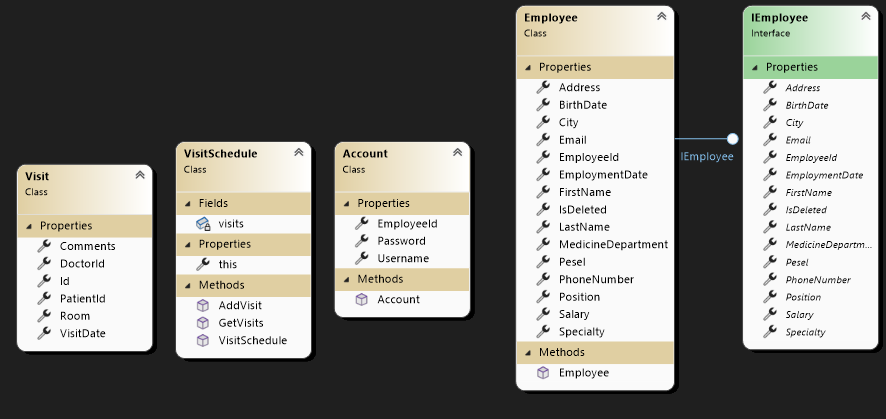
\includegraphics[height=8cm]{images/diag_gl_kl.png}
        \caption{Diagram głównych klas}
        \label{fig:diag_gl_kl}
    \end{center}
    \end{figure}

    \begin{figure}[H]
    \centering
    \subfigure{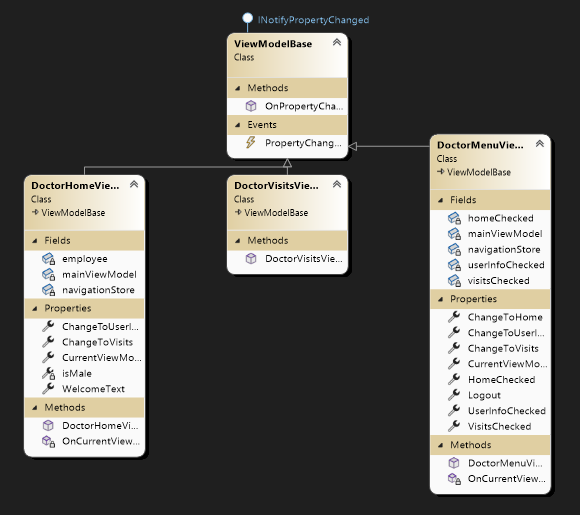
\includegraphics[width=0.4\textwidth]{images/diag_kl_nav_dok.png}} 
    \subfigure{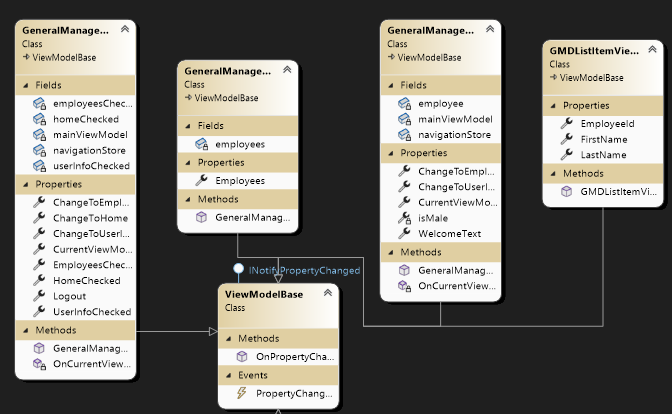
\includegraphics[width=0.5\textwidth]{images/diag_kl_nav_gen_man.png}} 
    \caption{Diagram klas nawigacyjnych dla 1)doktora 2)głównego kierownika}
 
    \label{fig:diag_kl_nav_dok_gl_kier}
    \end{figure}

    \begin{figure}[H]
    \centering
    \subfigure{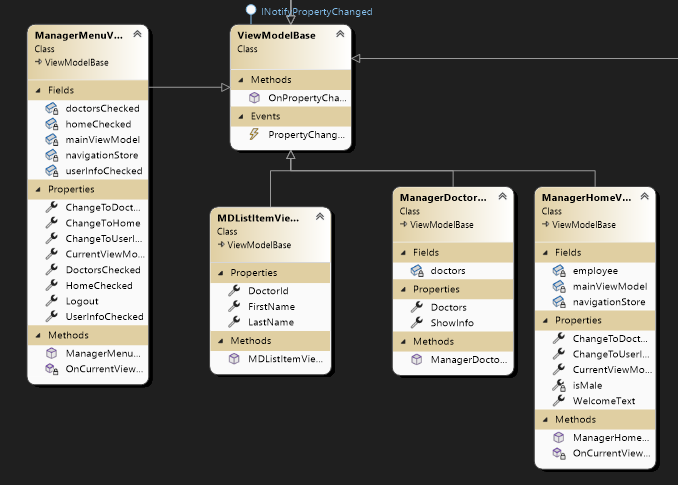
\includegraphics[width=0.4\textwidth]{images/diag_kl_nav_mang.png}} 
    \subfigure{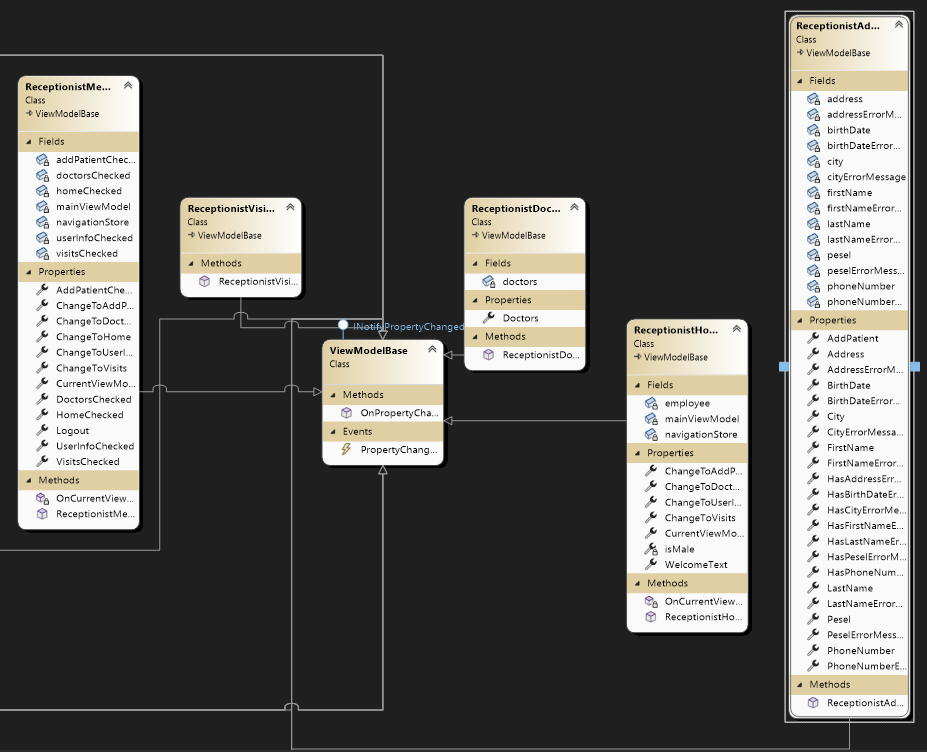
\includegraphics[width=0.4\textwidth]{images/diag_kl_nav_recep.png}} 
    \caption{Diagram klas nawigacyjnych dla 1)kierownika 2)recepcjonisty}
 
    \label{fig:diag_kl_nav_mang_recep}
    \end{figure}

    \begin{figure}[H]
    \begin{center}
	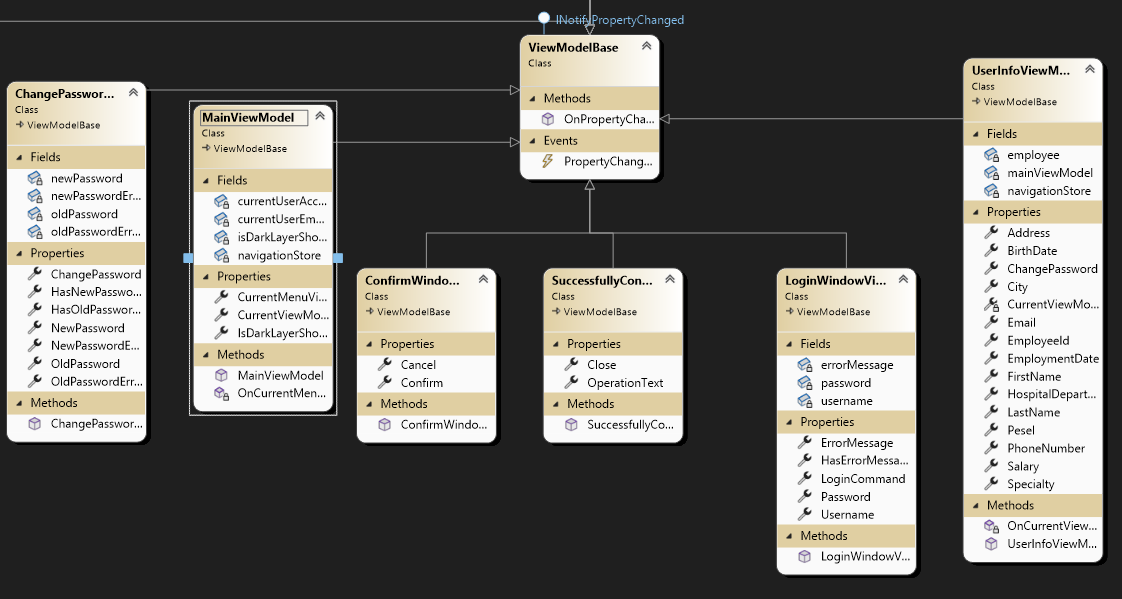
\includegraphics[height=7cm]{images/diag_kl_nav_wszt.png}
        \caption{Diagram klas nawigacyjnych dla wszystkich klientów}
        \label{fig:diag_kl_nav_recep}
    \end{center}
    \end{figure}
    
    \begin{figure}[H]
    \begin{center}
	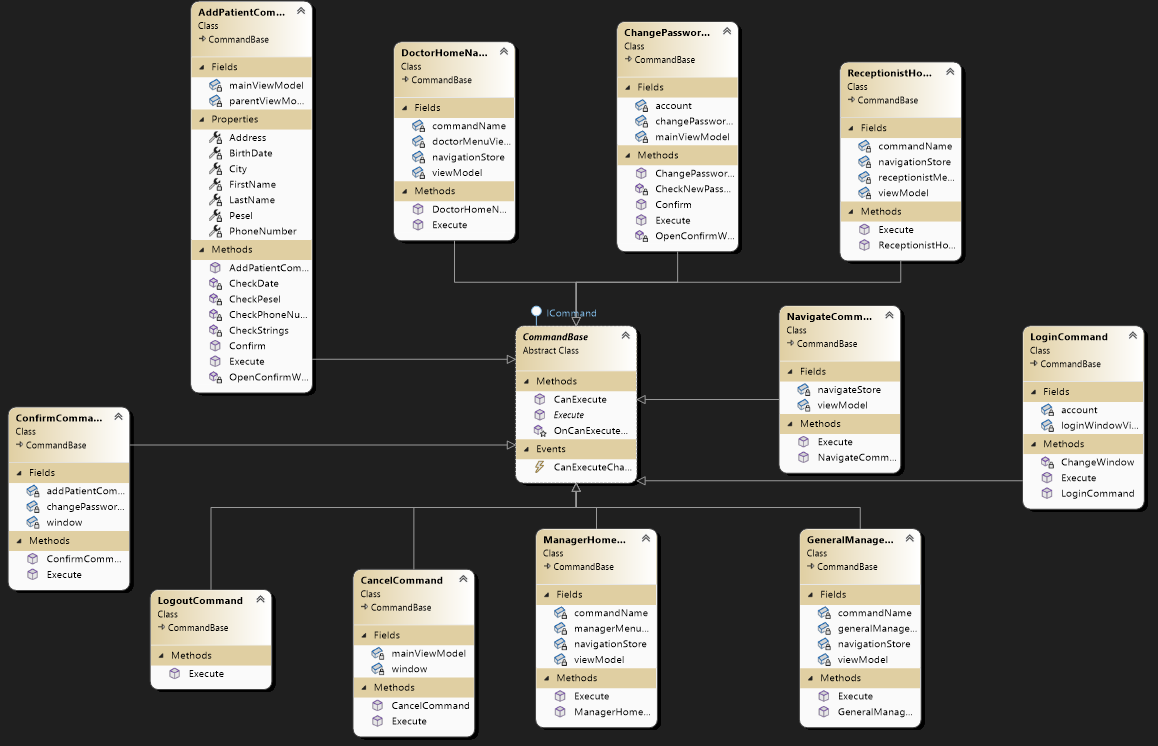
\includegraphics[height=7cm]{images/diag_kl_kom.png}
        \caption{Diagram klas komend}
        \label{fig:diag_kl_kom}
    \end{center}
    \end{figure}

    \begin{figure}[H]
    \begin{center}
	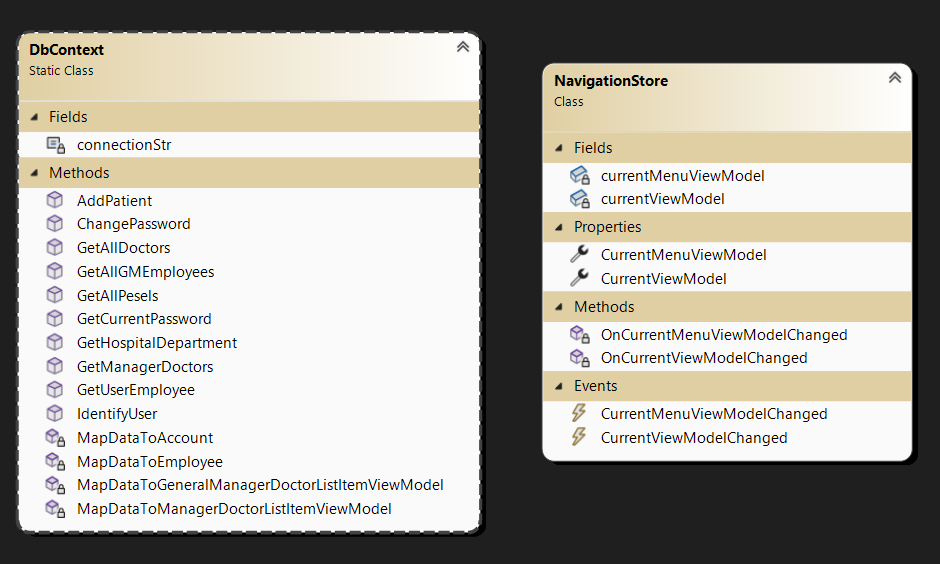
\includegraphics[height=5cm]{images/diag_kl_db_nav.png}
        \caption{Diagram klas dla bazy danych i przechowywania nawigacji}
        \label{fig:diag_kl_kom}
    \end{center}
    \end{figure}
    \subsection{\Large{Krótki opis}}
    \hspace{5mm} Projekt składa się z kilku części: Klasy główne(Models), Klasy używane do nawigacji i 
    Klasy główne używane są do przechowywania danych z bazy(np. Pracownik lub Wizyta). Klasy nawigacyjne używane są do przechowywania danych i operacji nad danymi pobranych od użytkownika w widoku(View) lub z bazy danych(np. UserInfoViewModel przechowuje informacje pobraną z bazy danych i przenosi ją do UserInfoView).
    Komendy wykorzystane są do nawigacji, przesłania danych do bazy danych lub otrzymania danych.
\end{flushleft}

% *************** Opis techniczny ***************
\begin{flushleft}
\section{\LARGE{Opis techniczny}}
\end{flushleft}

\begin{flushleft}
    \subsection{\Large{Narzędzie}}
    \hspace{5mm}Do tworzenia aplikacji \textquotedbl Szpital+\textquotedbl{} korzystałem z narzędzi {\color{blue}\href{https://pl.wikipedia.org/wiki/Windows_Presentation_Foundation}{WPF(Windows Presentation Foundation)}}. Jest to narzędznie do trowrzenia aplikacji desktopowych dla systemów Windows na bazie {\color{blue}\href{https://pl.wikipedia.org/wiki/.NET_Framework}{.Net Framework}}. Wykorzystywuje język opisy interfejsu użytkownika({\color{blue}\href{https://pl.wikipedia.org/wiki/Extensible_Application_Markup_Language}{XAML}}\label{href:XAML}) oraz język programowania {\color{blue}\href{https://pl.wikipedia.org/wiki/C_Sharp}{C\#}}\label{href:c_sh} do implementacji funkcjonalności elementów i innych funckji backend.
    \\
    \hspace{5mm} Dodatkowo przestrzegałem {\color{blue}\href{https://en.wikipedia.org/wiki/Model%E2%80%93view%E2%80%93viewmodel}{wzóru architektonicznego MVVM}}(Model-View-ViewModel)\label{href:MVVM}. Jest to wzór który rozdziela graficzny interfejs użytkownika GUI(View) od implementacji logiki biznesowej oraz logiki backend. Związkiem między tymi warstami jest konwerter wartości (ViewModel), który przyjmuje publiczne właściwości modeli(Models) i przekazuje ich do widoków(Views) za pomocą wiązania (Binding).
    \\
    \hspace{5mm} Do pisania kodu korzystałem z środowiska programistycznego {\color{blue}\href{https://pl.wikipedia.org/wiki/Microsoft_Visual_Studio}{Microsoft Visual Studio}\label{href:VStudio}}.
    \\
    \hspace{5mm}Także wykorzystełem wtyczki \textquotedbl {\color{blue} \href{https://github.com/charri/Font-Awesome-WPF}{FontAwesome.WPF}}\textquotedbl{} dla dodania ikon jako tekstu dla nawigacji bocznej i wtyczki \textquotedbl {\color{blue}\href{https://github.com/dotnet/corefx}{System.Data.SqlClient}}\textquotedbl{} dla połączenia z bazą danych SQL.
\end{flushleft}

\begin{flushleft}
    \subsection{\Large{Minimalne wymagania sprzętowe}}
    \begin{itemize}
        \item System operacyjny: Microsoft Windows 10 lub wyżej
        \item Procesor: x86 lub x64 z szybkością > 800 MHz
        \item RAM: 512 MB
        \item Miejsca na dysku: 25 MB
        \item Zainstalowany .Net 8.0
    \end{itemize}
\end{flushleft}

\begin{flushleft}
    \subsection{\Large{Baza danych}}
    \hspace{5mm}Do stworzenia i zarządzania bazą danych wykorzystywałem {\color{blue}\href{https://en.wikipedia.org/wiki/SQL_Server_Management_Studio}{Microsoft SQL Server Management Studio}}. Na lokalnym serwerze stworzyłem bazę danych "Spzital" (Rys.~\ref{fig:db_diag}). Także uzupełniłem bazę losowymi wartościami i dodałem kilka ograniczeń. Na przykład ograniczenie na wprowadzenie do nr\_grabinetu w wizycie większego od 127.
    \begin{figure}[H]
	\begin{center}
	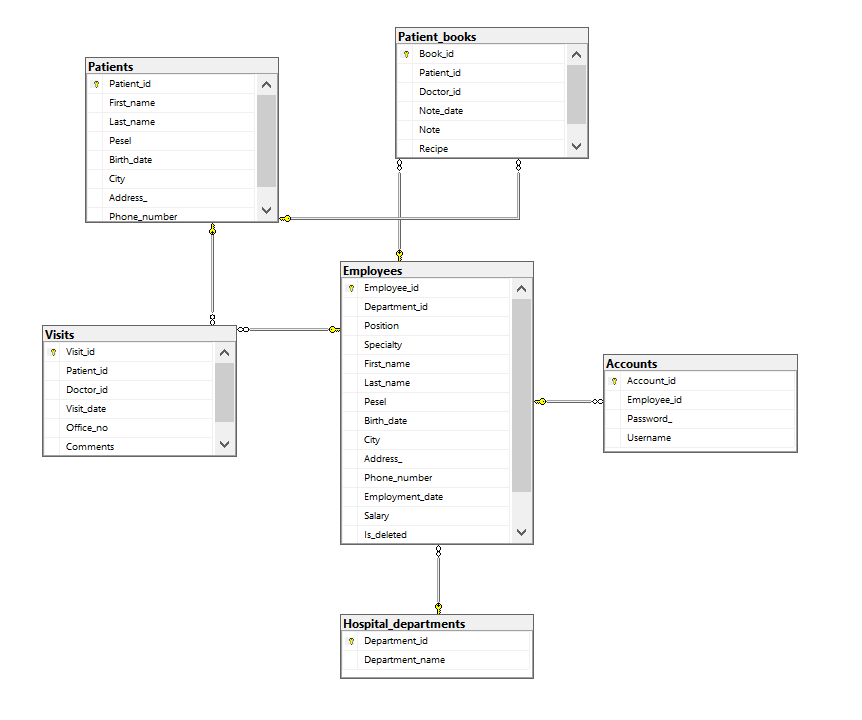
\includegraphics[width=10cm, height=10cm]{images/db_diagram.png}
        \caption{Diagram bazy danych}
        \label{fig:db_diag}
	\end{center}
    \end{figure}
    
    \hspace{5mm} Do pobrania danych z bazy do aplikacji wykorzystywuję klasy statycznej DbContext(Rys.~\ref{fig:db_c_k}) w której są metody robiące zapytania na bazę danych i wracające wartości pobrane z bazy.
    \begin{figure}[H]
    \centering
    \subfigure{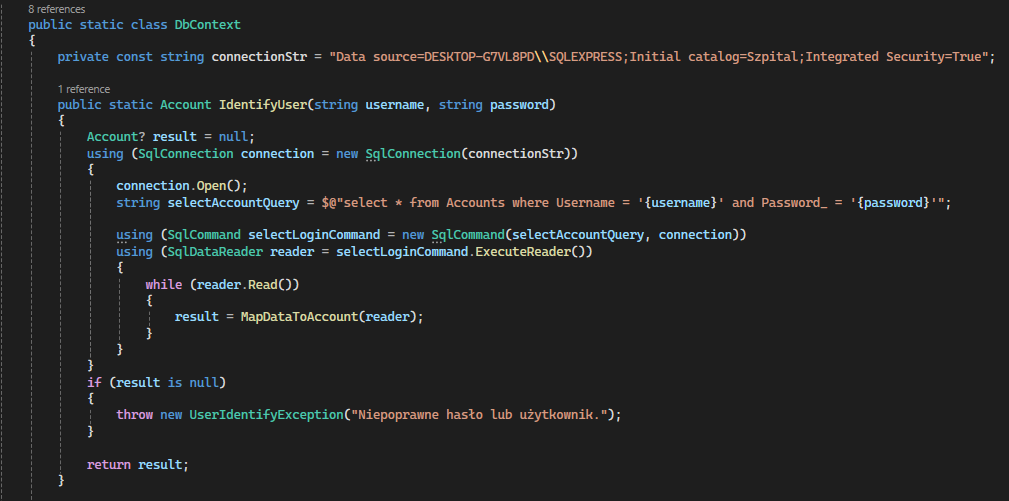
\includegraphics[width=0.6\textwidth]{images/db_cont_klas1.png}} 
    \subfigure{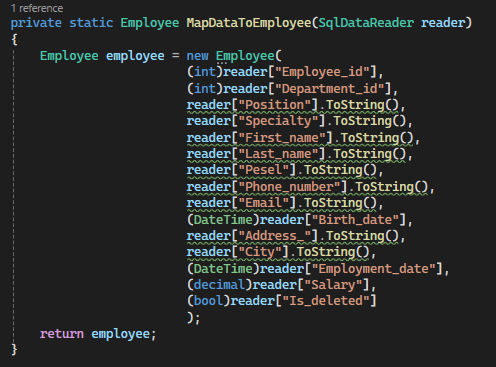
\includegraphics[width=0.38\textwidth]{images/db_cont_klas2.png}} 
    \caption{Klasa do zarządzania bazą danych(Przykładowa metoda)}
 
    \label{fig:db_c_k}
    \end{figure}
\end{flushleft}

% *************** Harmonogram realizacji projektu ***************
\begin{flushleft}
\section{\LARGE{Harmonogram realizacji projektu}\label{sec:harmon_proj}}
\end{flushleft}

\begin{figure}[H]
    \begin{center}
	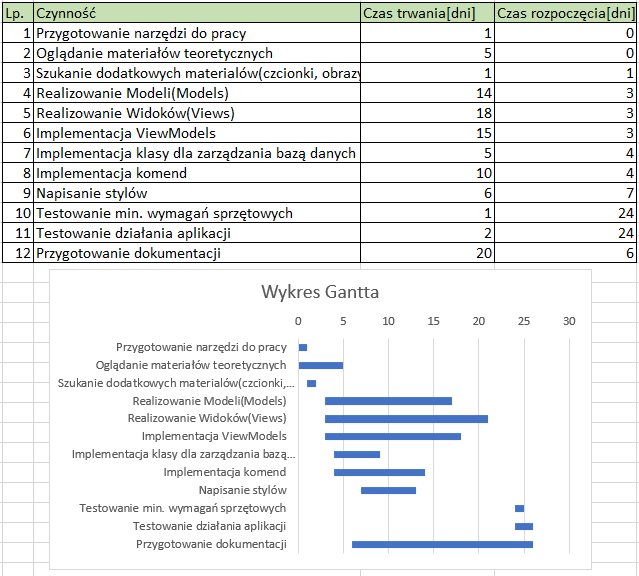
\includegraphics[height=10cm]{images/Wykres_Gantta.png}
        \caption{Wykres Gantta}
        \label{fig:wykr_gant}
    \end{center}
\end{figure}

% *************** Repozytorium ***************
\begin{flushleft}
\section{\LARGE{Repozytorium}}
\end{flushleft}

\begin{flushleft}
    \hspace{5mm}Do kontroli wersji oraz przechowywania wykorzystałem systemu Git oraz serwisu internetowego GitHub.
    \\
    \hspace{5mm}Wszystkie pliki źródłowe projektu oraz dokumentacji są umieszczone w tym linku - {\color{blue}\href{https://github.com/clowd1e/Szpital}{Repozytorium GitHub}}.
\end{flushleft}
\newpage

% *************** Prezentacja ***************
\begin{flushleft}
\section{\LARGE{Prezentacja}}
\end{flushleft}

\begin{flushleft}
    \subsection{\Large{Logowanie}}
    \hspace{5mm}Uruchomiwszy aplikację, użytkowniku wyświetla się okno logowania:
    \begin{figure}[H]
	\begin{center}
	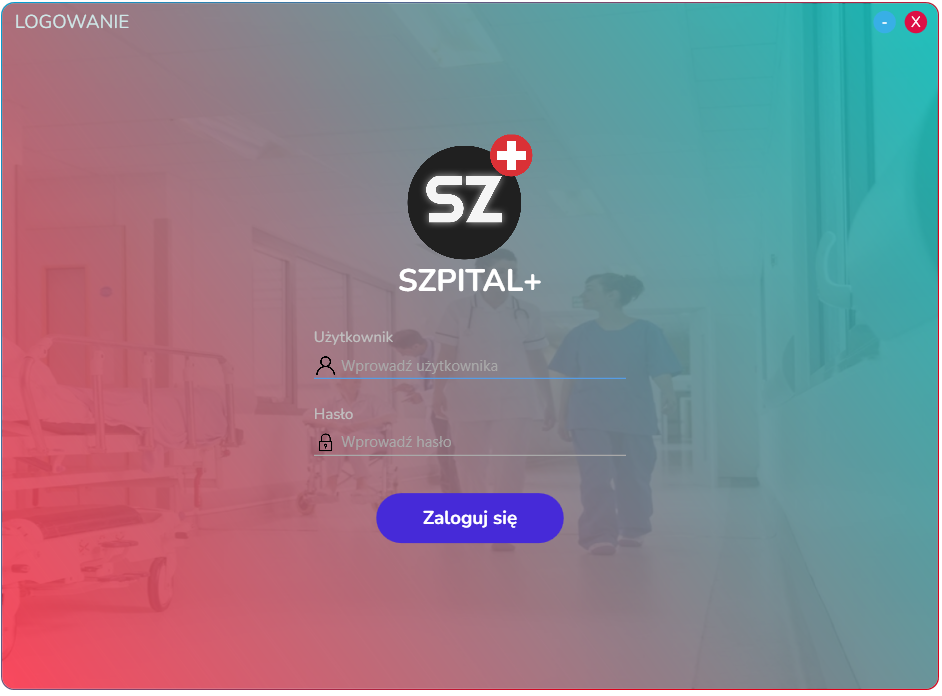
\includegraphics[height=7cm]{images/log_widok.png}
        \caption{Okno logowania}
        \label{fig:okn_log}
	\end{center}
    \end{figure}
    \hspace{5mm}W tym oknie został przerobiony górny standardowy panel aplikacji windows. Rozmiar okna 750x550px. Także tło oraz granica zrobione z gradientu. Okno jest trochę zaokrąglone. Po wprowadzeniu danych i naciśnięciu przycisku \textquotedbl Zaloguj się\textquotedbl{} klasa statyczna DbContext sprawdza czy użytkownik istnieje i czy hasło jest poprawne za pomocą polecenia SQL. W przypadku gdy użytkownik poda błędne dane DbContext rzuca wyjątek \textquotedbl UserIdentifyException\textquotedbl{} który jest łapany w LoginCommand, skąd wypisuje się komunikat.
    \begin{figure}[H]
	\begin{center}
	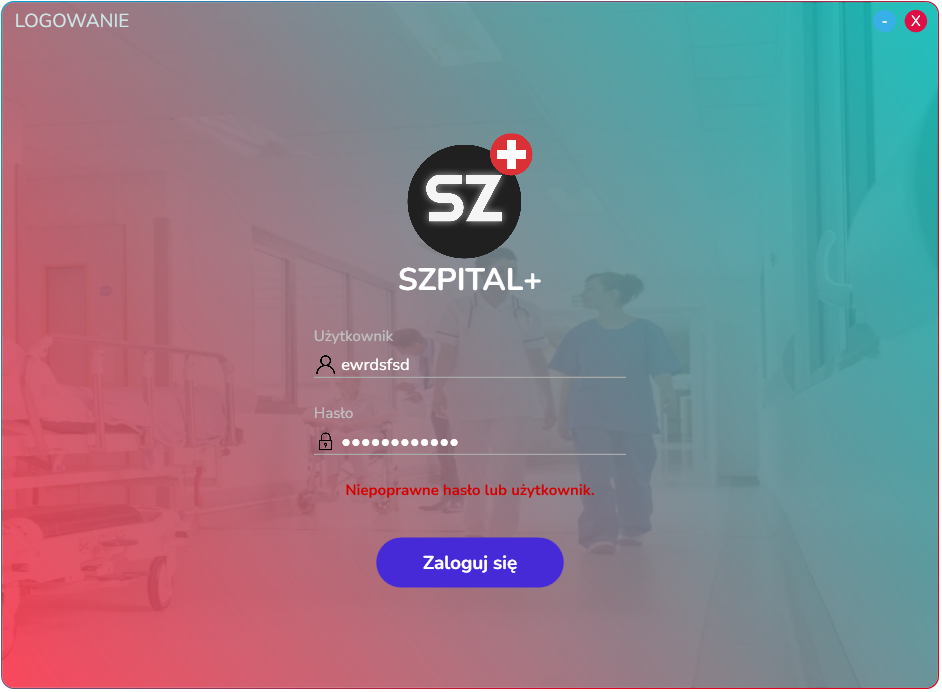
\includegraphics[height=8cm]{images/niep_uzyt.png}
        \caption{Wprowadzenie błędnych danych do logowania}
        \label{fig:okn_log}
	\end{center}
    \end{figure}
    \hspace{5mm}Jeśli użytkownik istnieje i hasło jest poprawne —logujemy się do aplikacji.
    \begin{figure}[H]
    \centering
    \subfigure{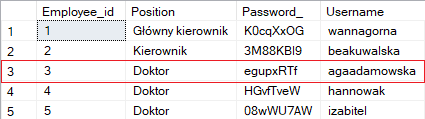
\includegraphics[width=0.7\textwidth]{images/istn_uzyt.png}} 
    \subfigure{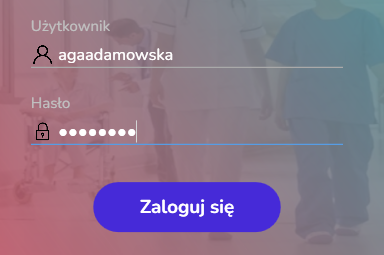
\includegraphics[width=0.3\textwidth]{images/rand_uzyt1.png}}
    \subfigure{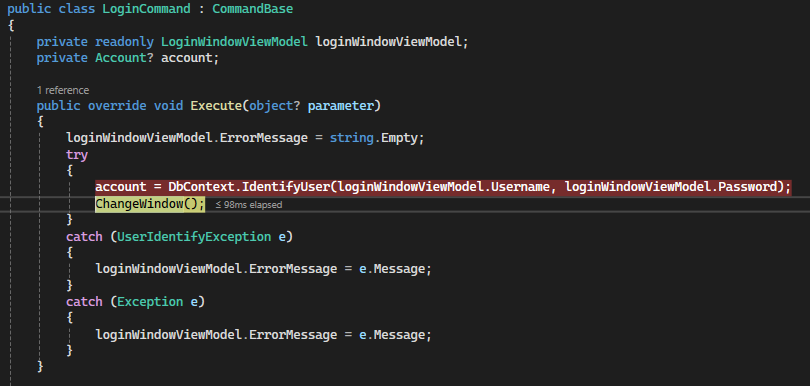
\includegraphics[width=0.5\textwidth]{images/log_kom_exe.png}}
    \caption{Logowanie (DbContext nie rzucił wyjątku)}
    \label{fig:popr_log}
    \end{figure}
    \subsection{\Large{Główne okno}}
    \hspace{5mm}MainWindow(Okno główne) składa się z trzech części:
    \begin{figure}[H]
	\begin{center}
	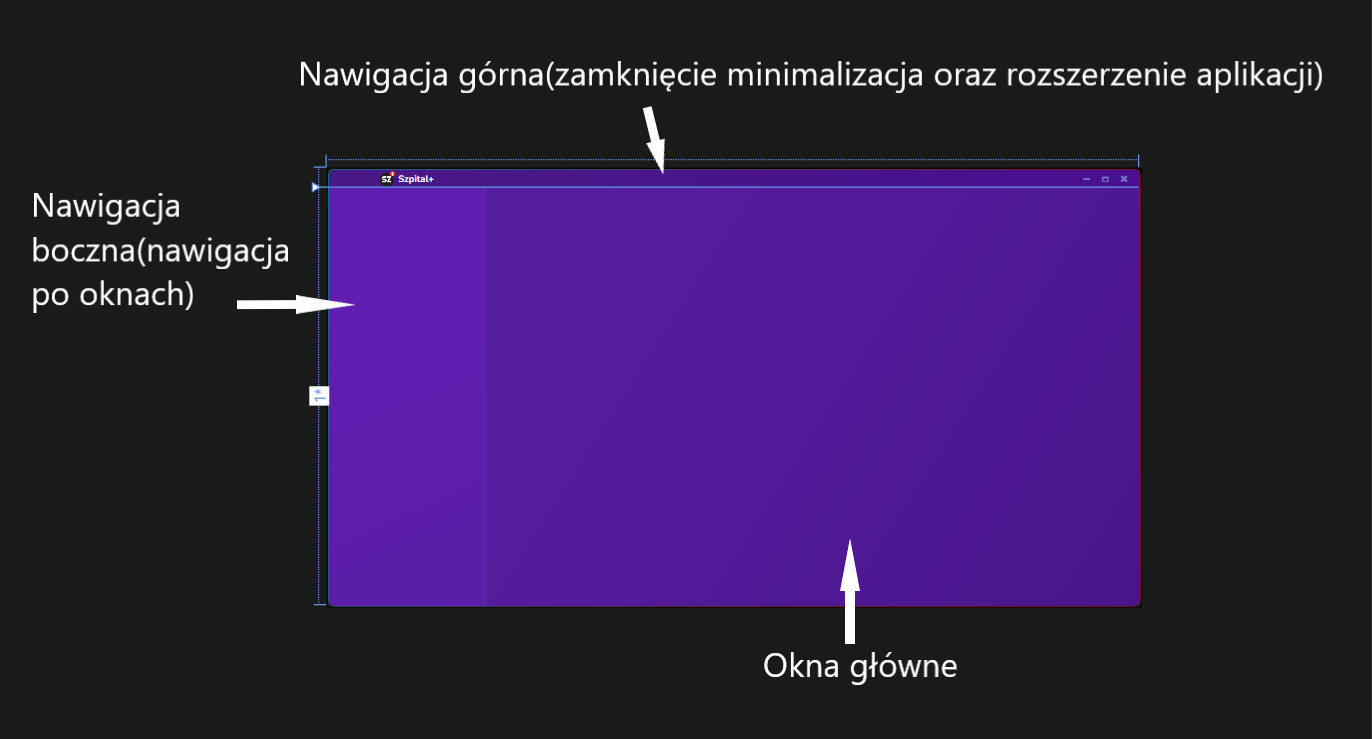
\includegraphics[height=8cm]{images/mainwindow.png}
        \caption{Główne okno}
        \label{fig:okn_glow}
	\end{center}
    \end{figure}
    \hspace{5mm}Aplikacja pobiera dane z bazy i ze względu na to, na jakim stanowisku pracuje użytkownik, wykorzystuje jeden z szablonów dotyczący jego posady żeby stworzyć nowy wygląd nawigacji bocznej.
    \begin{figure}[H]
	\begin{center}
	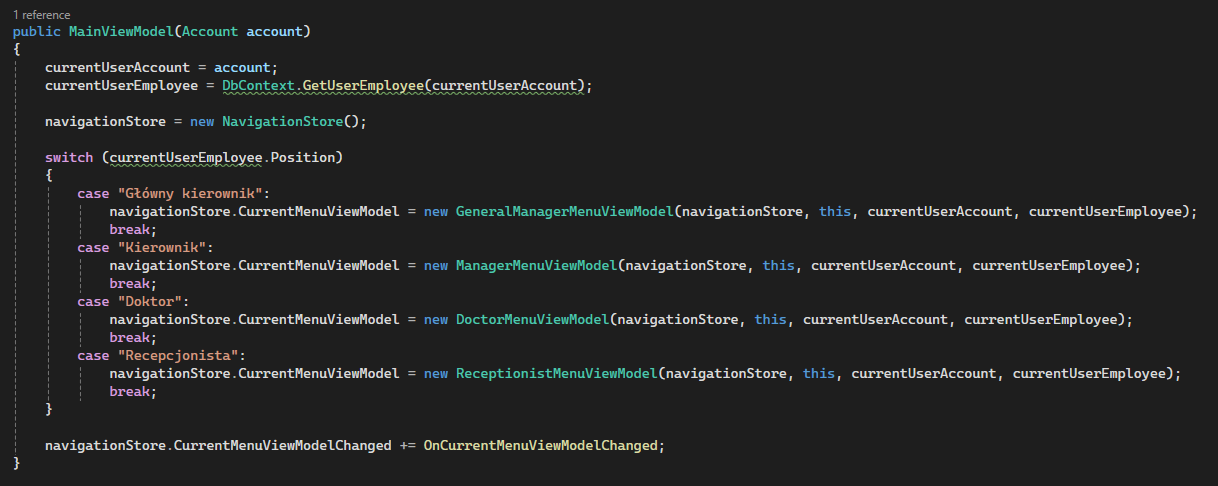
\includegraphics[height=5cm]{images/mainviewmodel_const.png}
        \caption{Pobieranie stanowiska użytkownika i przypisanie nowego wyglądu}
        \label{fig:main_vm_const}
	\end{center}
    \end{figure}
    \hspace{5mm}Na przykład do aplikacji został zalogowany Recepcjonista.
    Wtedy wygląd jego aplikacji będzie następny(także aplikacja sprawdza jaki zwrot wykorzystać na pulpicie ze względu na płeć osoby):
    \begin{figure}[H]
	\begin{center}
	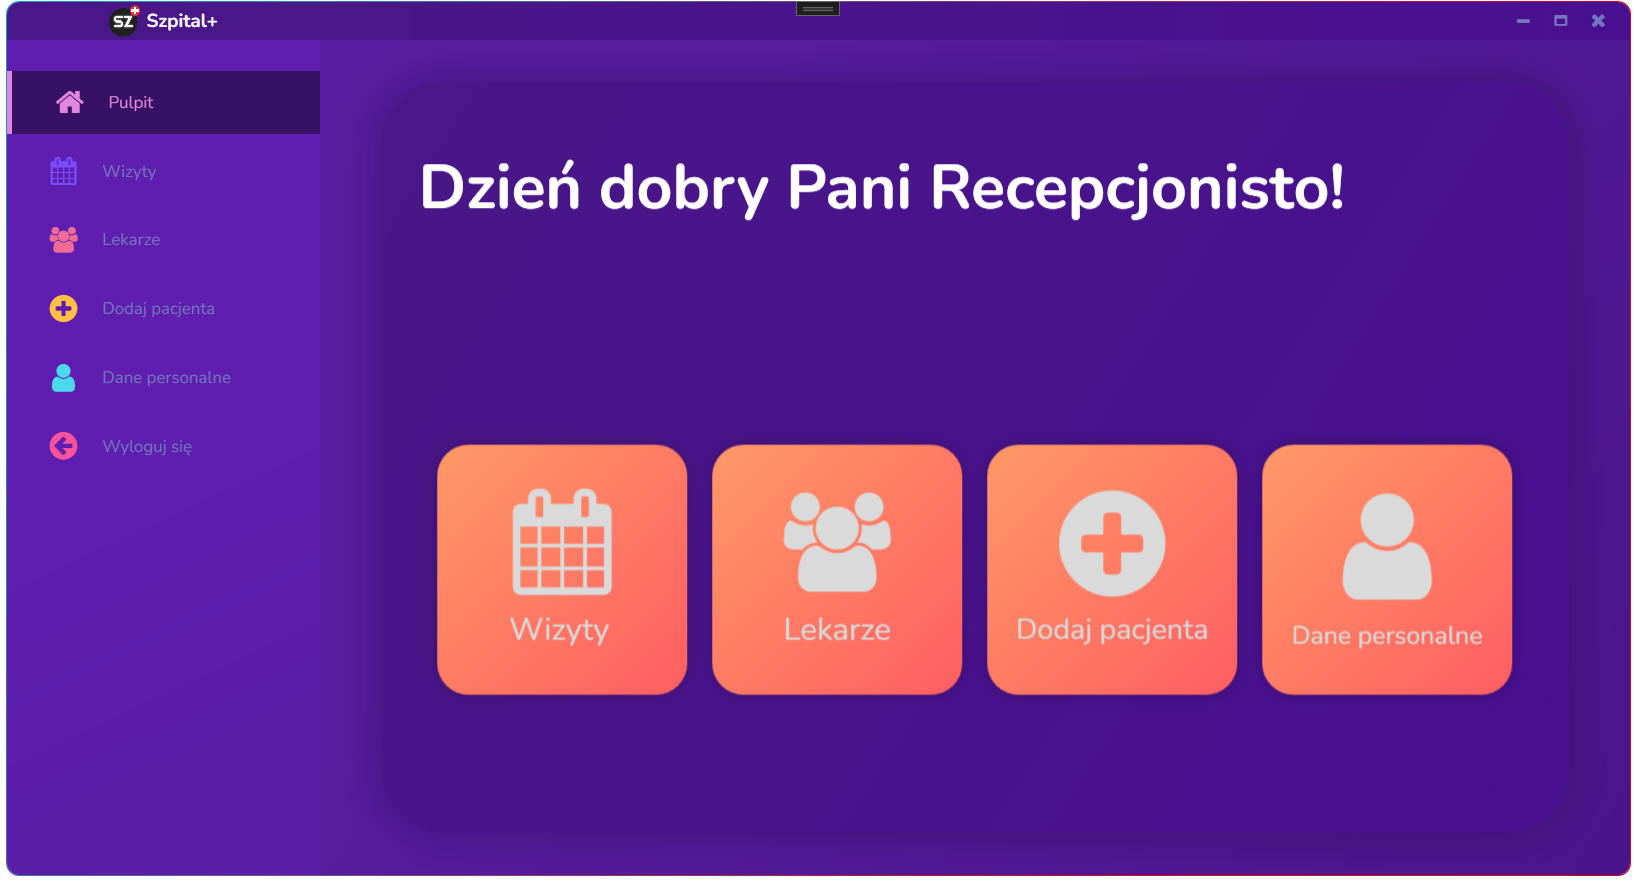
\includegraphics[height=7cm]{images/recep_view.png}
        \caption{Wygląd aplikacji recepcjonisty(Katarzyna Pabiniak)}
        \label{fig:recep_view}
	\end{center}
    \end{figure}
    \begin{figure}[H]
        \begin{center}
	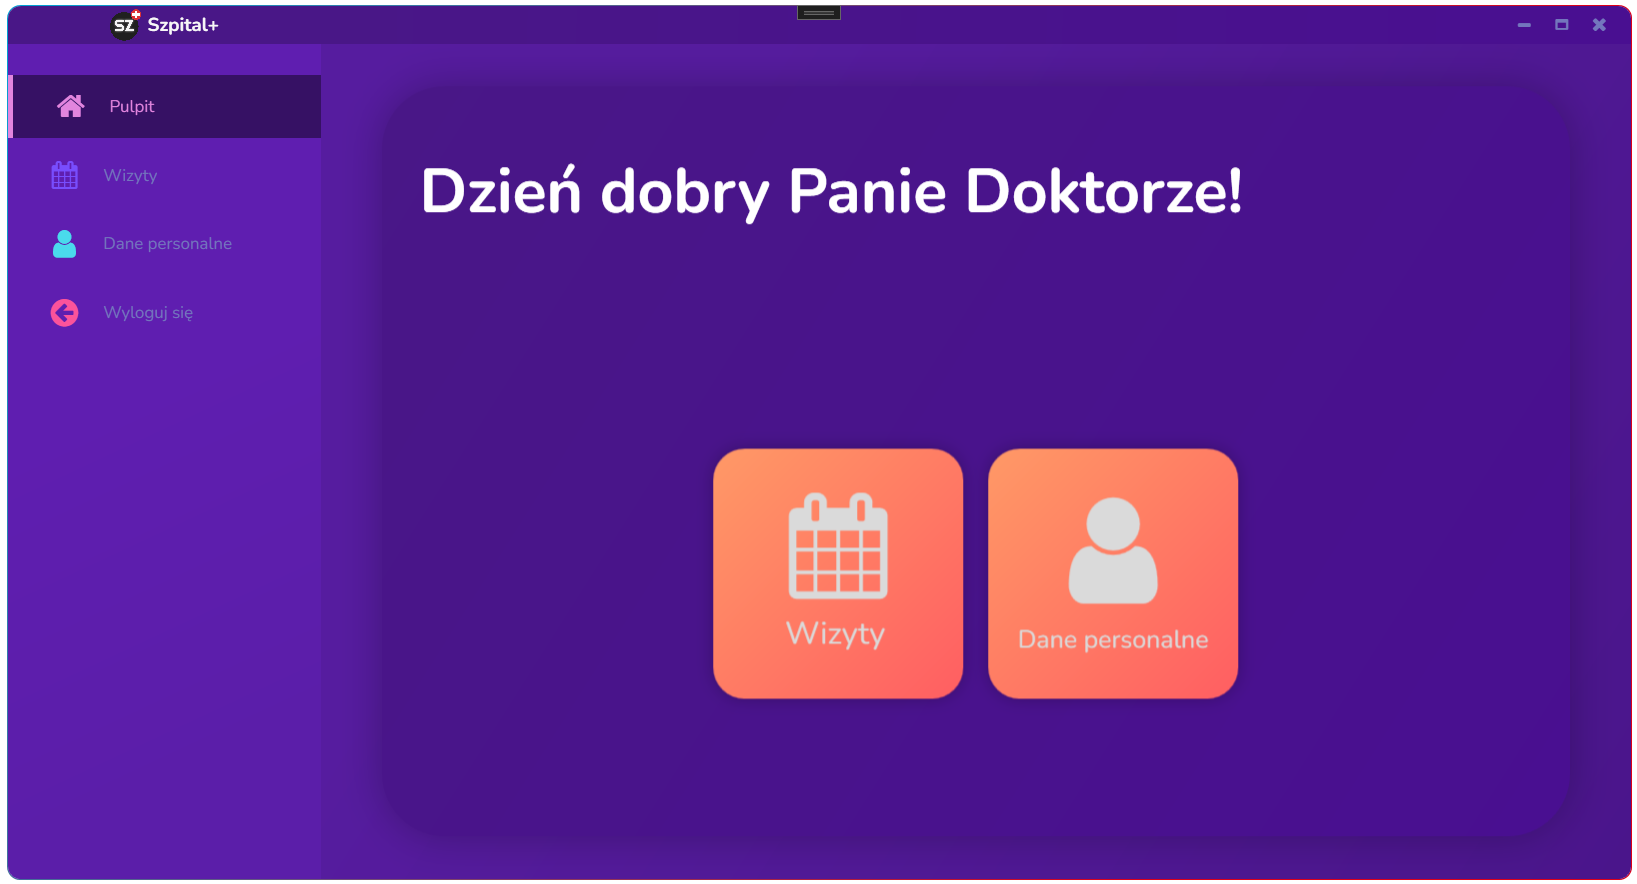
\includegraphics[height=7cm]{images/doktor_view.png}
        \caption{Wygląd aplikacji doktora(Filip Jabcoń)}
        \label{fig:doktor_view}
	\end{center}
    \end{figure}
    \hspace{5mm}Każdy klient na panelu nawigacyjnym bocznym ma przyciski: pulpit(okno z nawigacją), dane personalne(dane o użytkowniku), wyloguj się(wylogowanie z systemu i wracanie do okna logowania).
    \subsection{\Large{Dane personalne}}
    \begin{figure}[H]
    \centering
    \subfigure{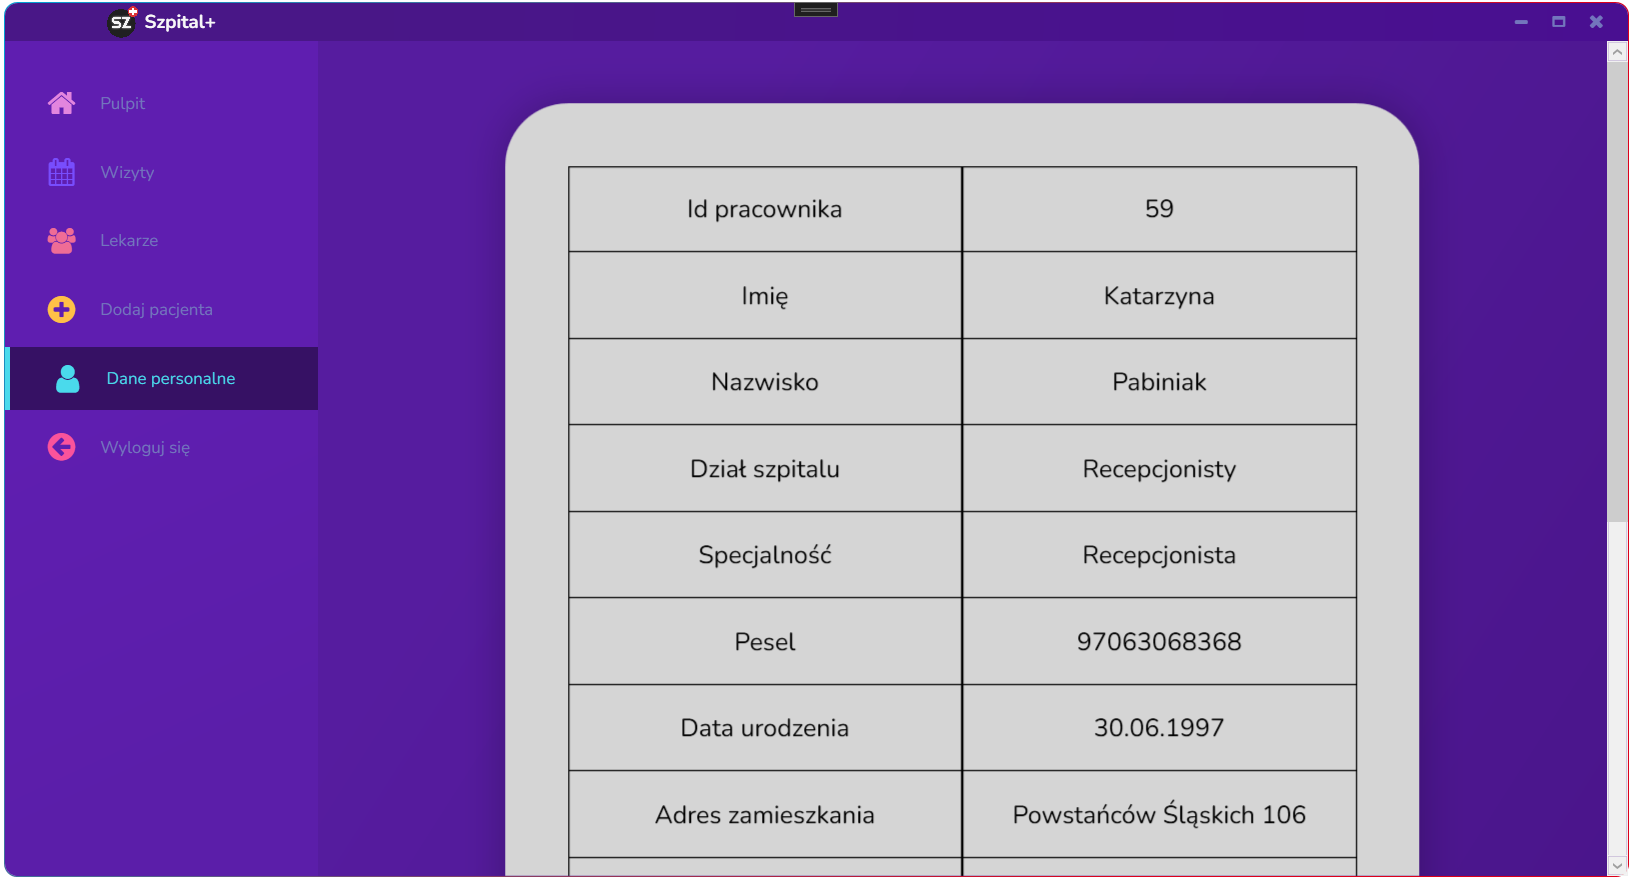
\includegraphics[width=0.7\textwidth]{images/dane_person1.png}} 
    \subfigure{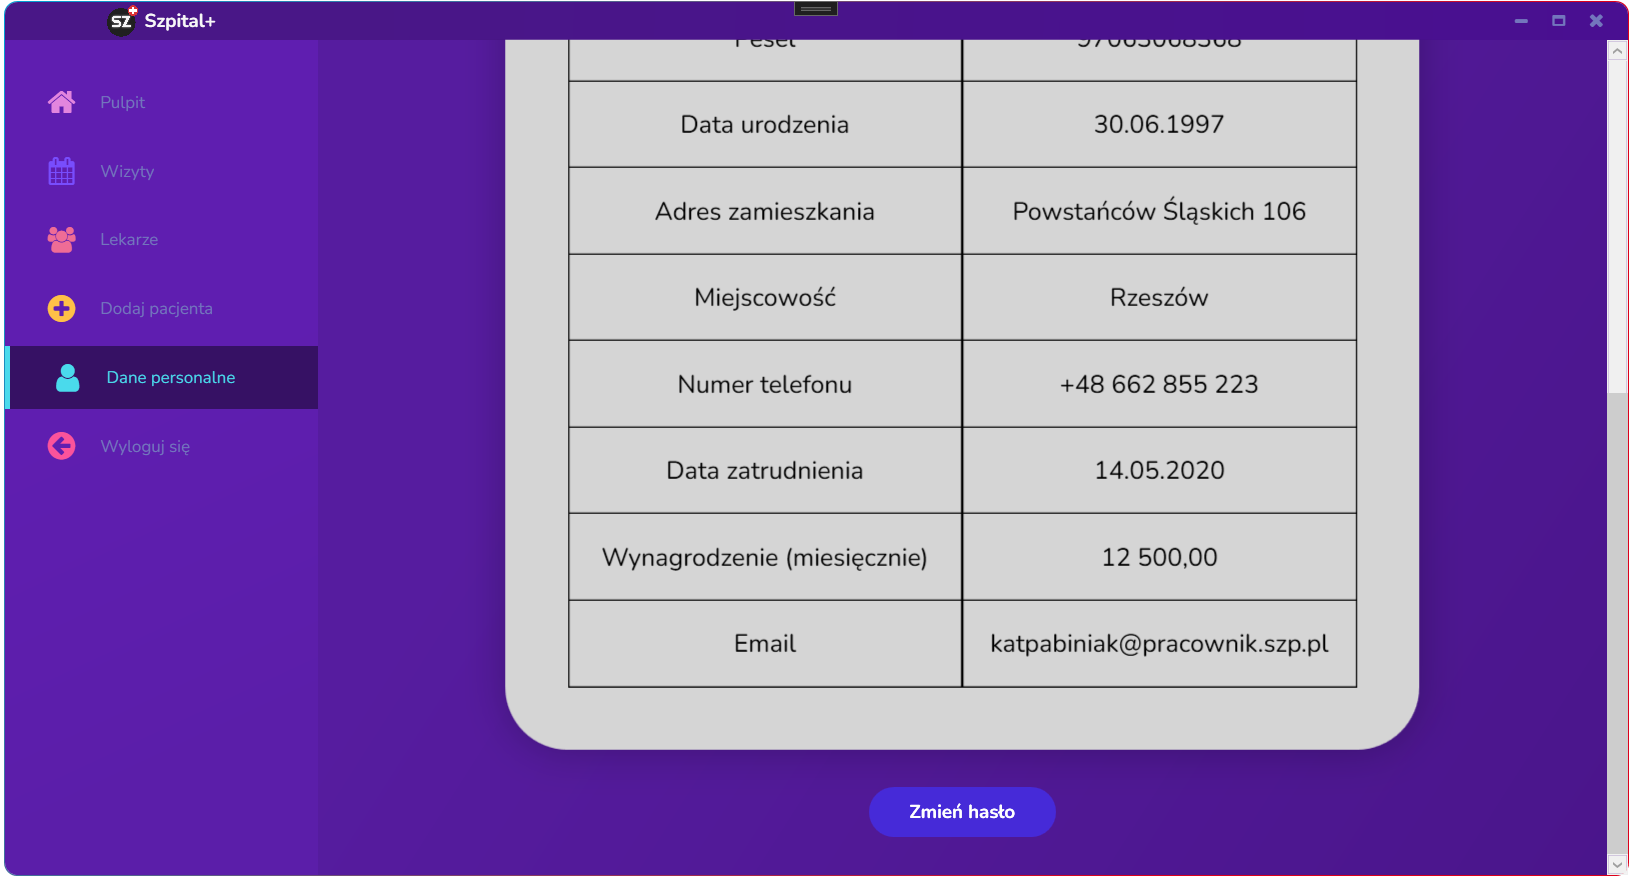
\includegraphics[width=0.7\textwidth]{images/dane_person2.png}}
    \caption{Wygląd danych personalnych}
    \label{fig:dane_person}
    \end{figure}
    \newpage
    \subsection{\Large{Zmienianie hasła}}
    \hspace{5mm}Zmienianie hasła dostępne na dołu okna Dane personalne za pomocą przycisku.
    \begin{figure}[H]
        \begin{center}
	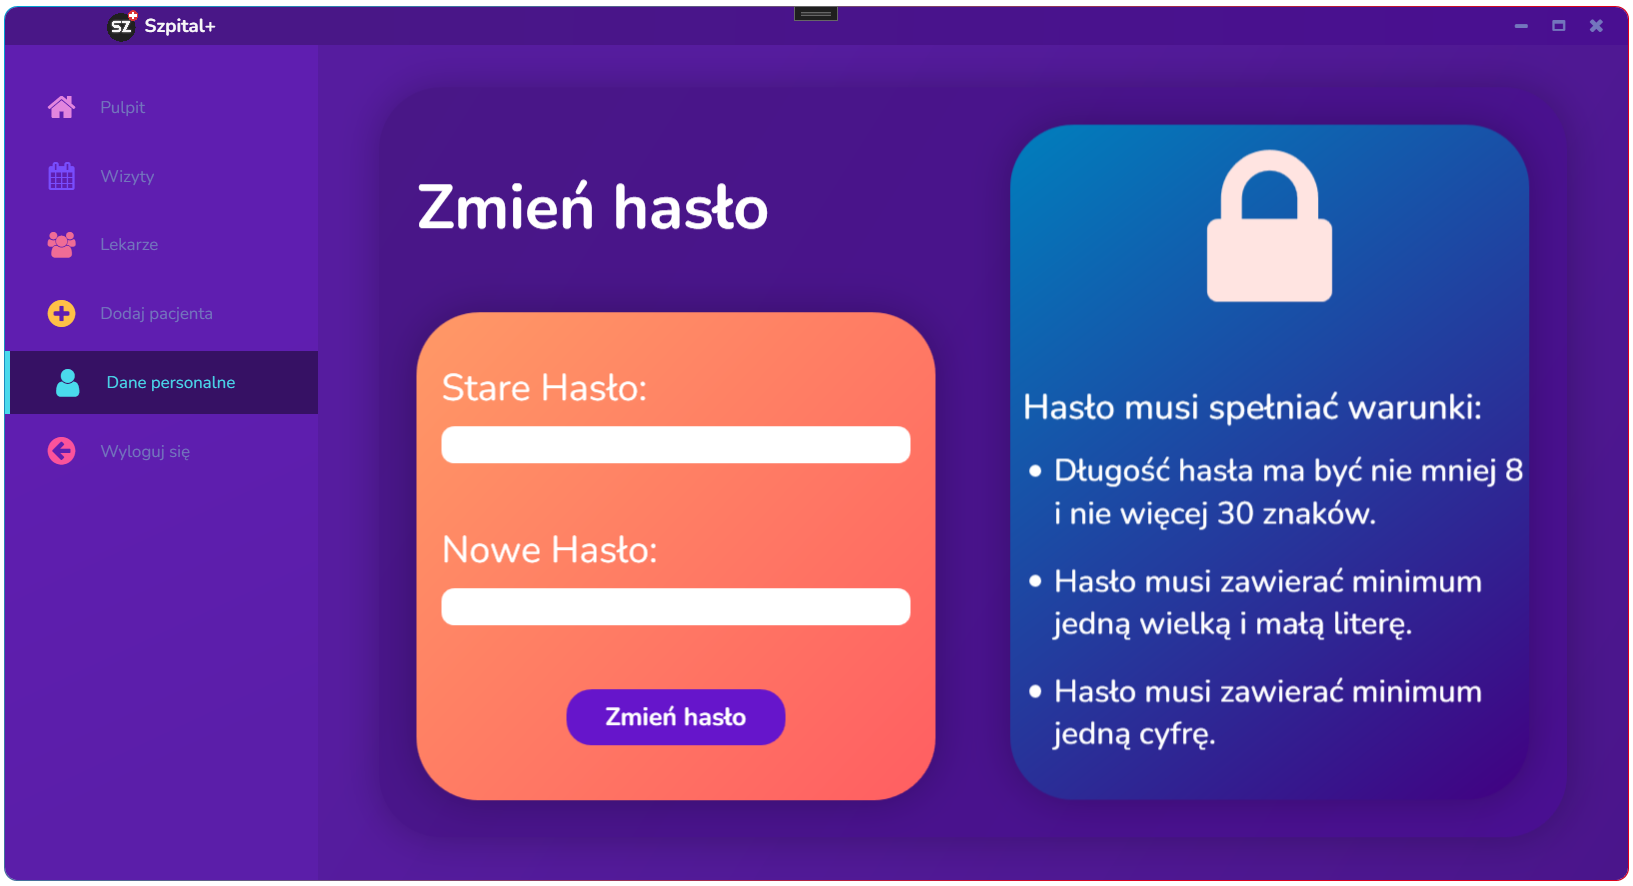
\includegraphics[height=7cm]{images/zmien_hasl.png}
        \caption{Wygląd okna \textquotedbl Zmień hasło\textquotedbl{}}
        \label{fig:zmien_hasl}
	\end{center}
    \end{figure}
    \hspace{5mm}Jeśli stare hasło nie będzie takim samym jak w bazie danych wystąpi błąd:
    \begin{figure}[H]
        \begin{center}
	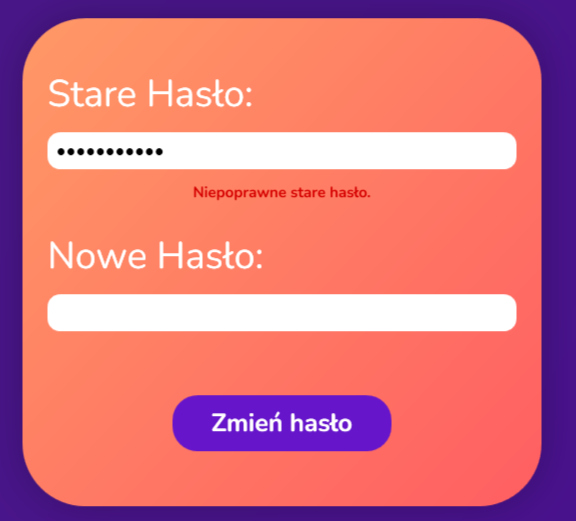
\includegraphics[height=5cm]{images/niepop_stare_hasl.png}
        \caption{Błąd przy wpisaniu starego hasła}
        \label{fig:niepop_st_haslo}
	\end{center}
    \end{figure}
    \newpage
    \subsubsection{\large{Sprawdzenie nowego hasła}}
    \hspace{5mm}Sprawdzenie nowego hasła odbywa się za pomocą {\color{blue}\href{https://en.wikipedia.org/wiki/Regular_expression}{wyrażenia regularnego}}({\color{blue}\href{https://learn.microsoft.com/en-us/dotnet/standard/base-types/regular-expression-language-quick-reference}{Klasa Regex}}).
    \begin{figure}[H]
        \begin{center}
	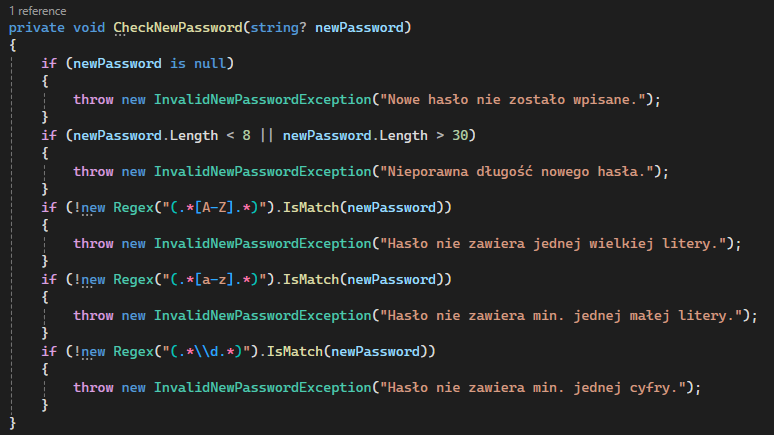
\includegraphics[height=6cm]{images/sprawdz_hasl.png}
        \caption{Metoda do sprawdzenia nowego hasła}
        \label{fig:sprawdz_hasl}
	\end{center}
    \end{figure}
    \begin{figure}[H]
        \begin{center}
	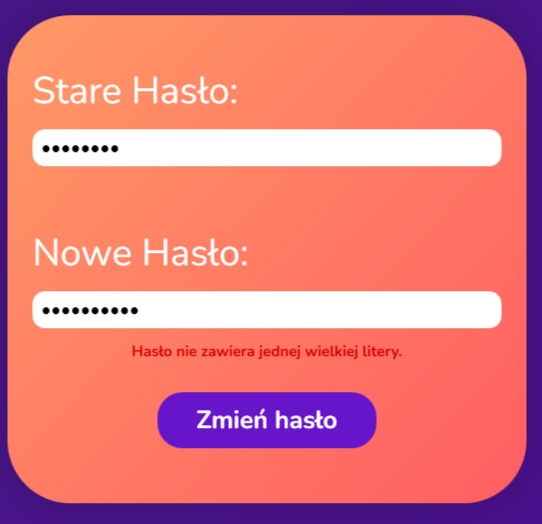
\includegraphics[height=6cm]{images/blad_nowe_hasl.png}
        \caption{Wystąpienie błędu przy nowym hasłu}
        \label{fig:blad_nowe_haslo}
	\end{center}
    \end{figure}
    \hspace{5mm}Jeśli nowe hasło odpowiada wszystkim warunkom, pojawia się okno do zatwierdzenia operacji. Przy tym interakcja z głownem oknem jest niemożliwa dopóki użykownik anuluje lub zatwierdzi operację.
    \begin{figure}[H]
        \begin{center}
	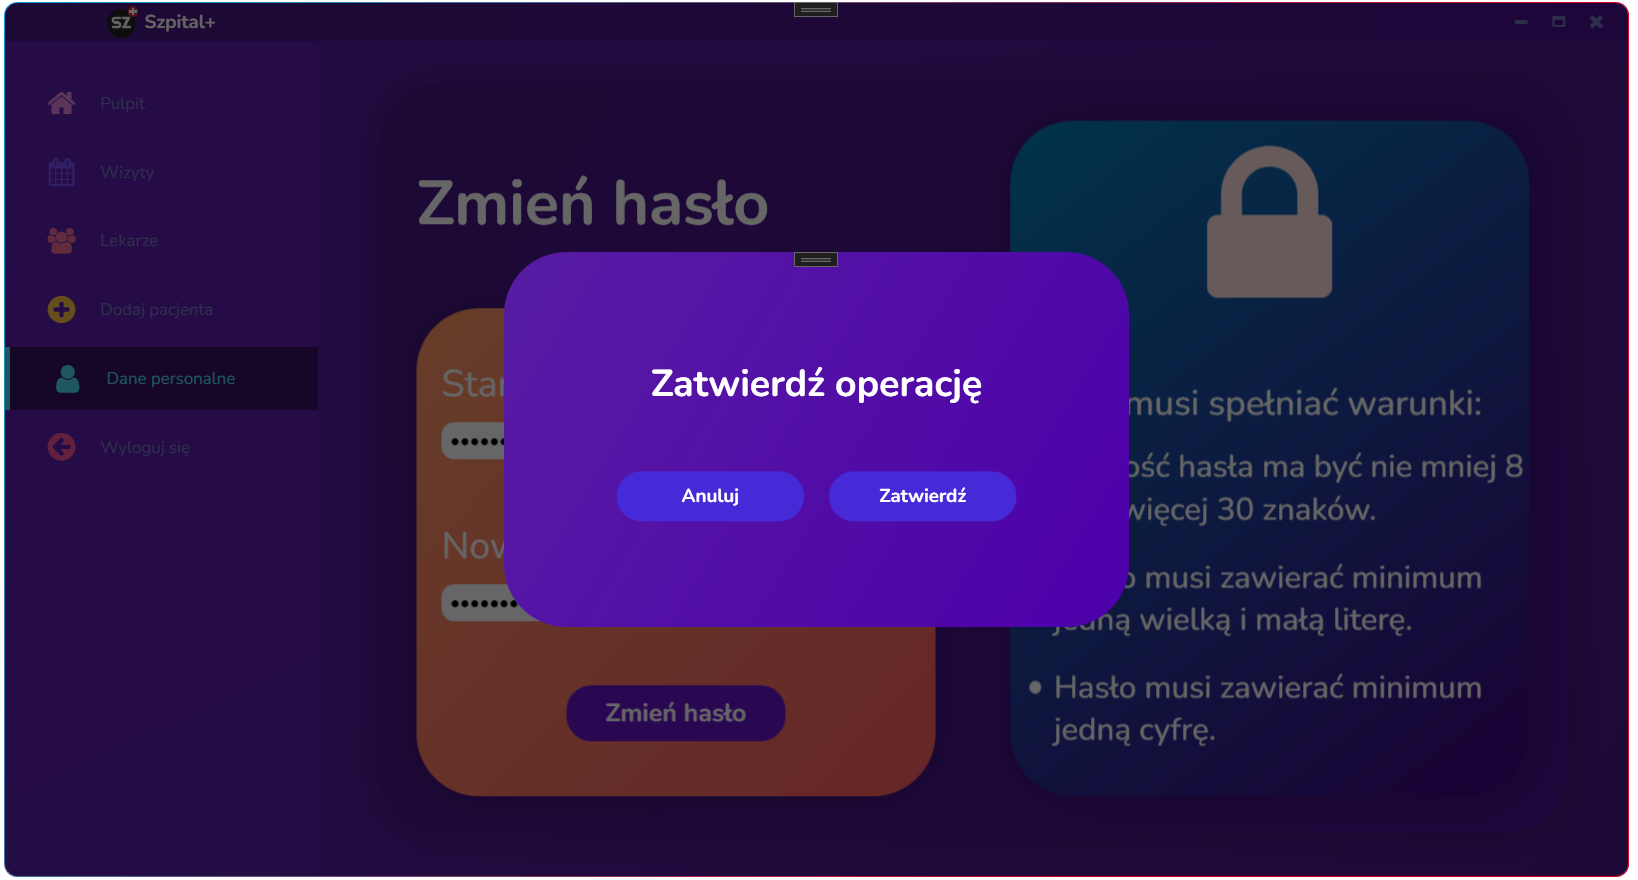
\includegraphics[height=6cm]{images/zatw_oper.png}
        \caption{Okno do zatwierdzenia operacji}
        \label{fig:zatw_oper}
	\end{center}
    \end{figure}
    \begin{figure}[H]
        \begin{center}
	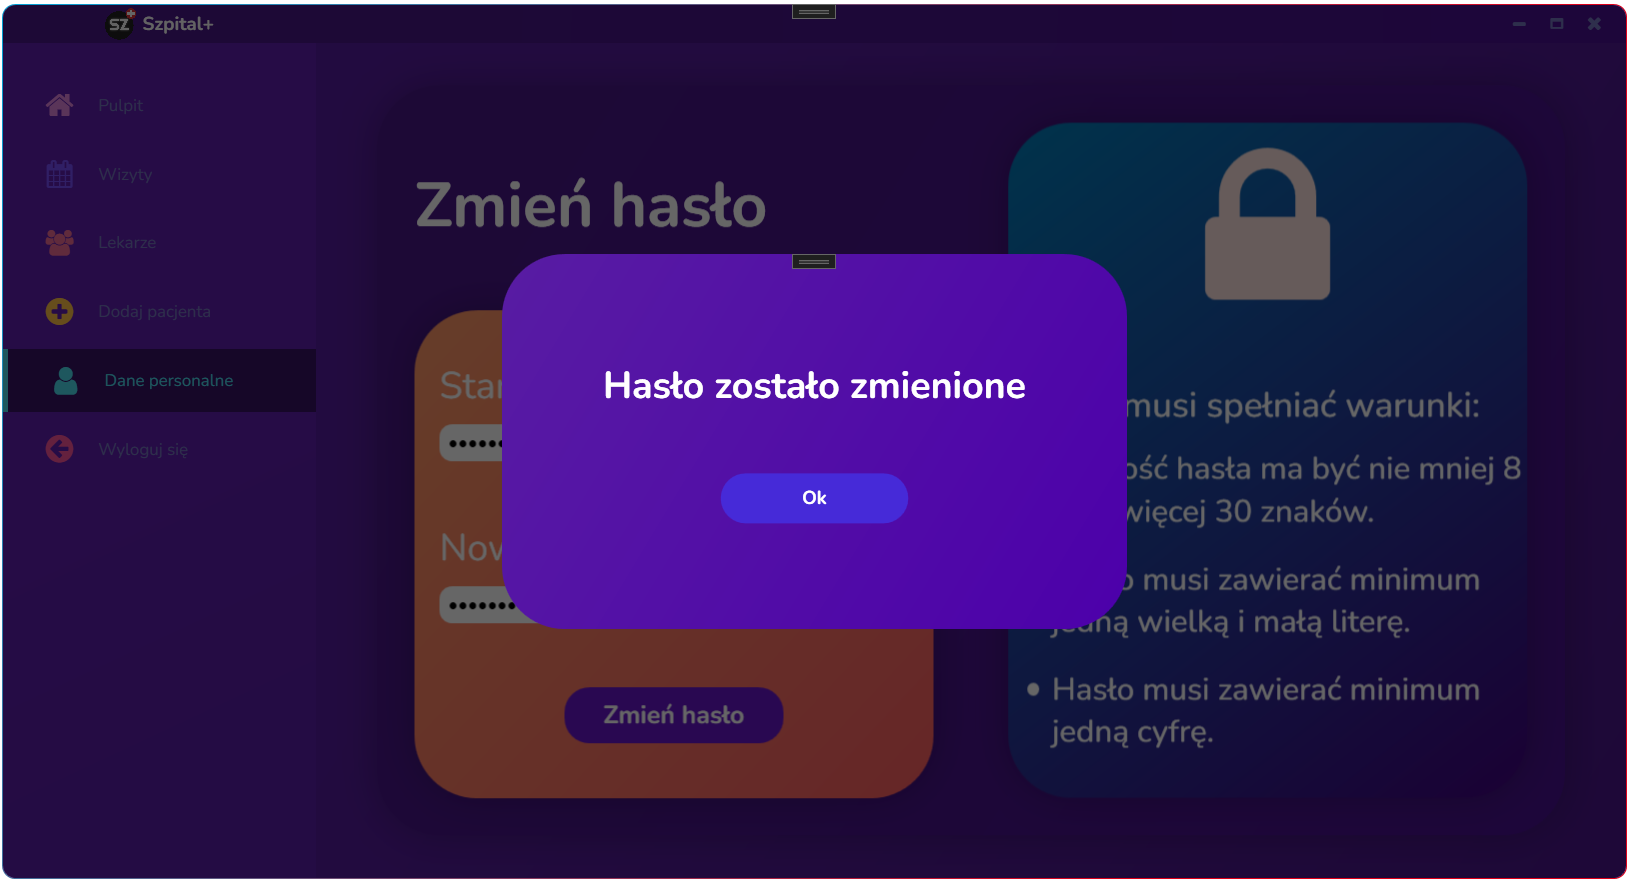
\includegraphics[height=6cm]{images/haslo_zos_zmien_katpa.png}
        \caption{Hasło zostało zmienione}
        \label{fig:haslo_zost_zmien}
	\end{center}
    \end{figure}
    \begin{figure}[H]
    \centering
    \subfigure{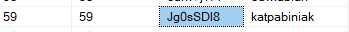
\includegraphics[width=0.4\textwidth]{images/stare_haslo_katpa.png}} 
    \subfigure{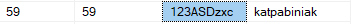
\includegraphics[width=0.4\textwidth]{images/nowe_haslo_katpa.png}}
    \caption{Nowe i stare hasło}
    \end{figure}
    \subsection{\Large{Okna dla recepcjonisty}}
    \subsubsection{\large{Wizyty - nie został zaimplementowany}}
    \subsubsection{\large{Lekarze}}
    \begin{figure}[H]
        \begin{center}
	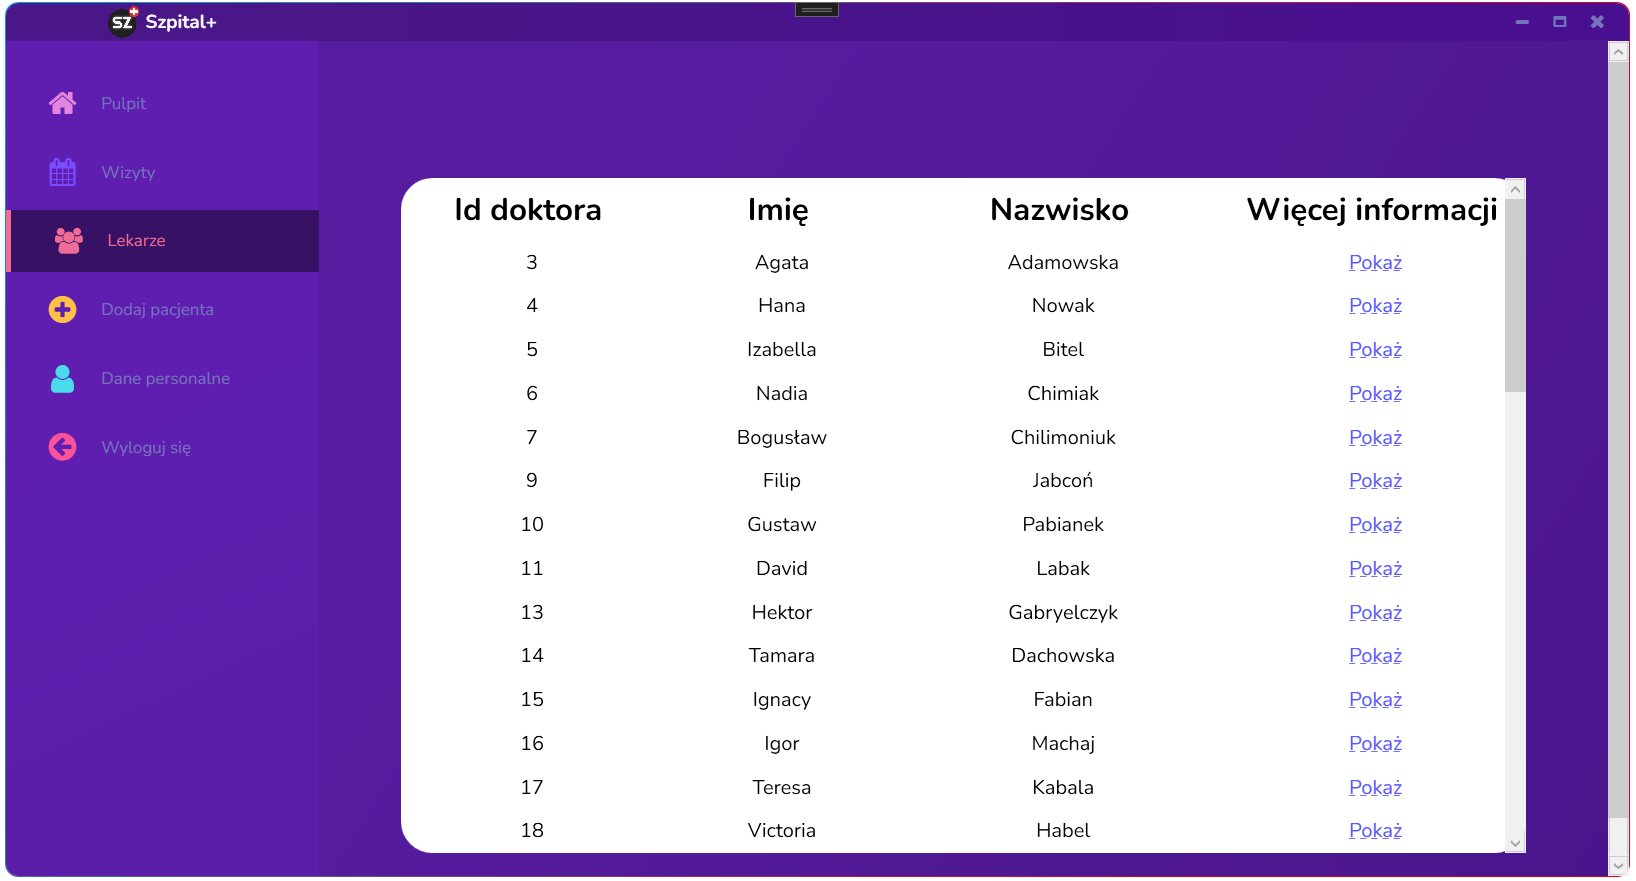
\includegraphics[height=7cm]{images/recep_lekarze.png}
        \caption{Okno recepcjonisty(Lekarze)}
        \label{fig:recep_lekarze}
	\end{center}
    \end{figure}
    \hspace{5mm}Przycisk \textquotedbl Pokaż\textquotedbl{} nie został zaimplementowany.
    \subsubsection{\large{Dodaj pacjenta}}
    \begin{figure}[H]
    \centering
    \subfigure{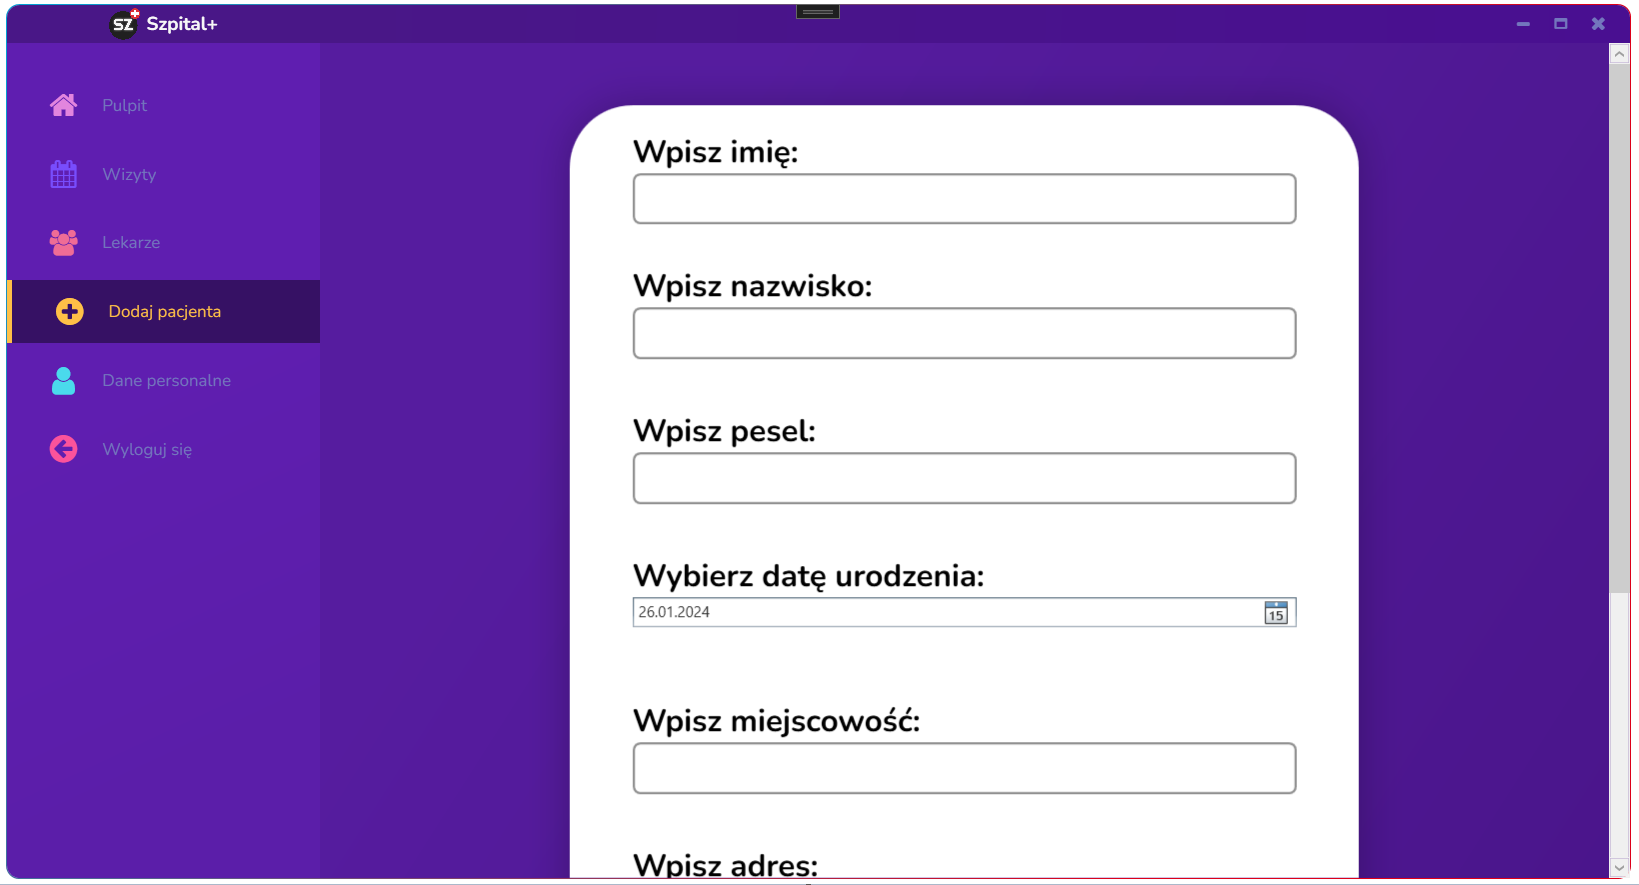
\includegraphics[width=0.5\textwidth]{images/dodaj_pacj_1.png}} 
    \subfigure{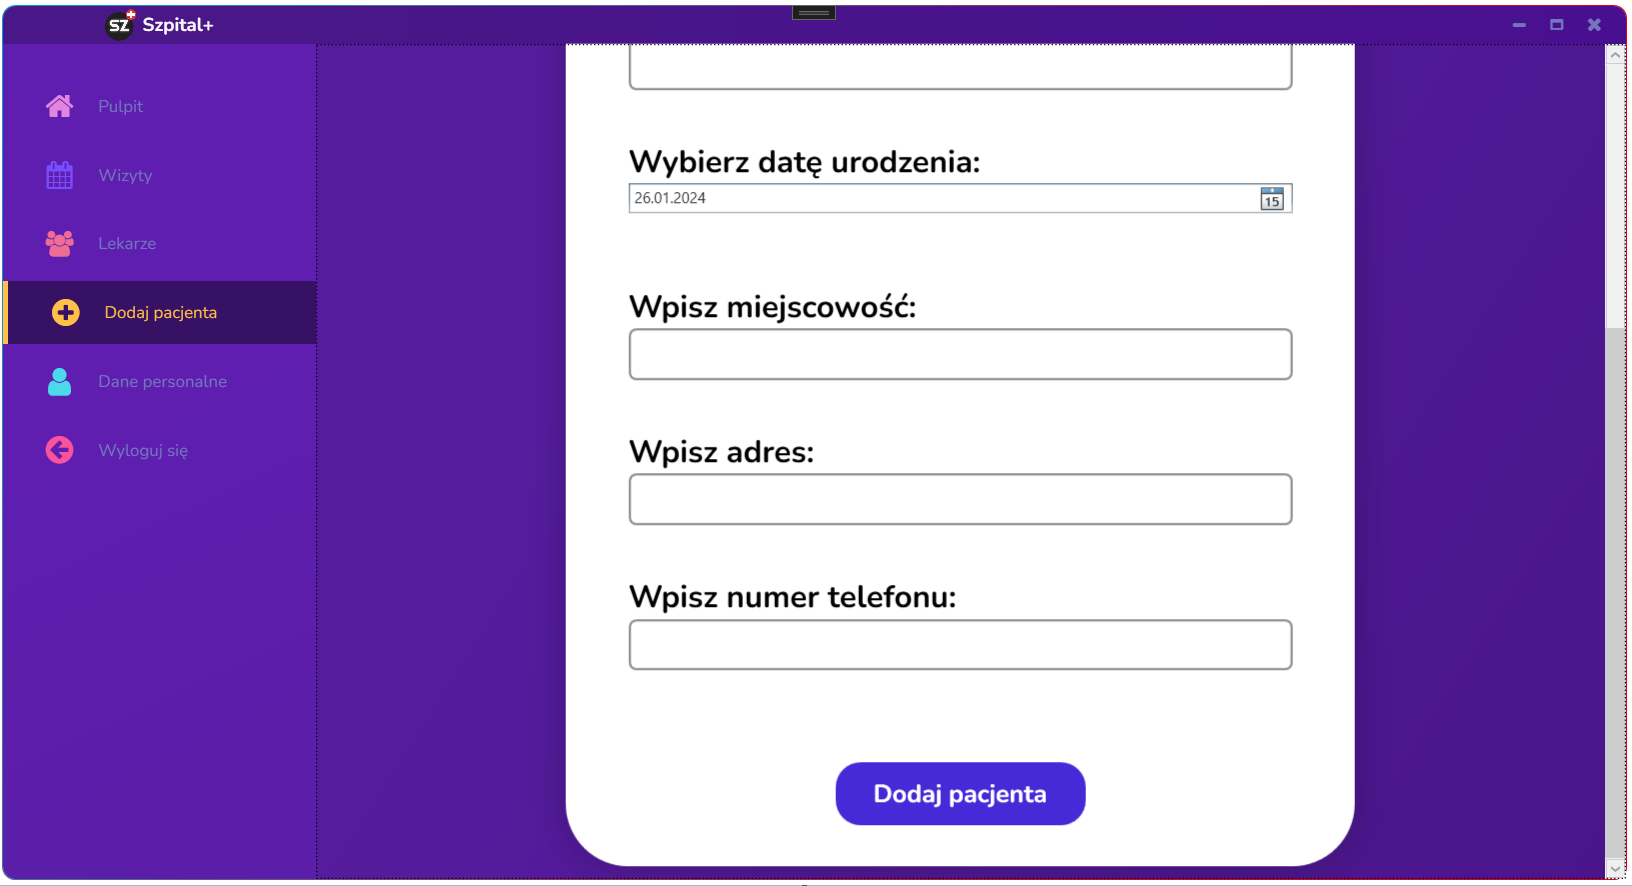
\includegraphics[width=0.5\textwidth]{images/dodaj_pacj_2.png}}
    \caption{Okno recepcjonisty(Dodaj pacjenta)}
    \end{figure}
    \begin{figure}[H]
        \begin{center}
	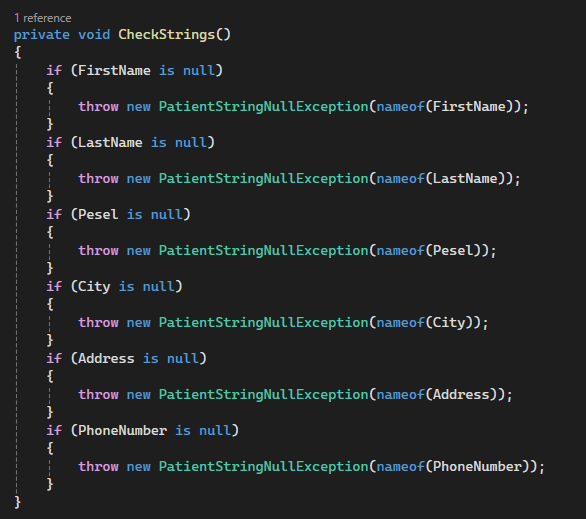
\includegraphics[height=7cm]{images/spraw_null.png}
        \caption{Sprawdzenie na puste pola}
        \label{fig:spraw_null}
	\end{center}
    \end{figure}
    \begin{figure}[H]
        \begin{center}
	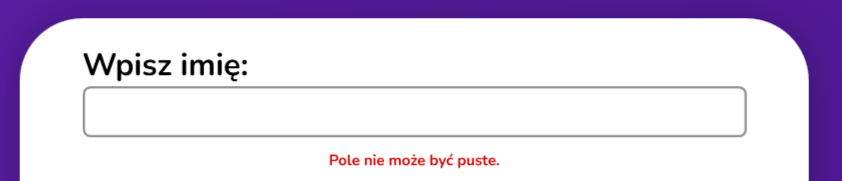
\includegraphics[height=3cm]{images/blad_wpisz_im.png}
        \caption{Wystąpienie błędu przy pustym błędzie}
        \label{fig:blad_wpisz_im}
	\end{center}
    \end{figure}
    \begin{figure}[H]
        \begin{center}
	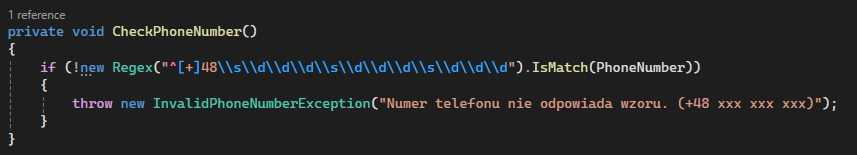
\includegraphics[height=3cm]{images/sprawd_telef.png}
        \caption{Sprawdzenie formatu telefonu}
        \label{fig:sprawd_telef}
	\end{center}
    \end{figure}
    \begin{figure}[H]
        \begin{center}
	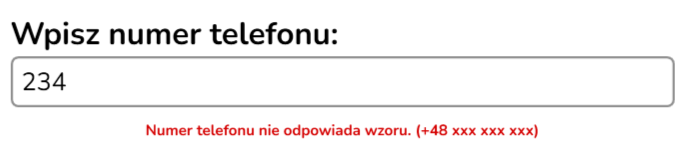
\includegraphics[height=3cm]{images/blad_telef.png}
        \caption{Błąd przy polu numeru telefonu}
        \label{fig:blad_telef}
	\end{center}
    \end{figure}
    \begin{figure}[H]
        \begin{center}
	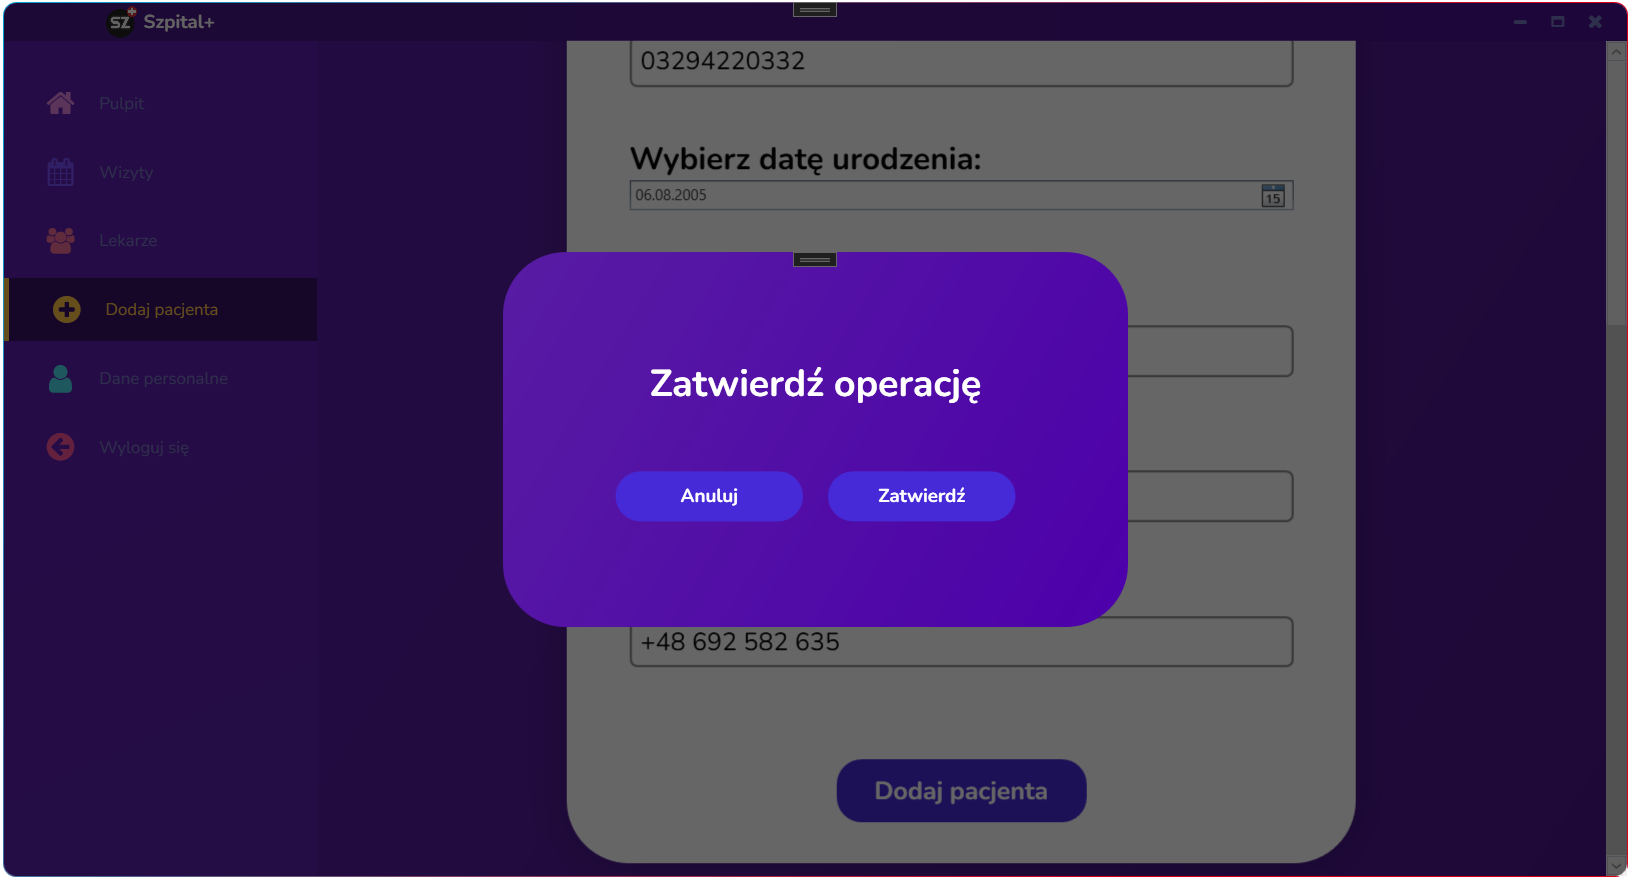
\includegraphics[height=6cm]{images/zatwr_oper_dod.png}
        \caption{Zatwierdzenie operacji}
        \label{fig:zatwr_oper_dod}
	\end{center}
    \end{figure}
    \begin{figure}[H]
        \begin{center}
	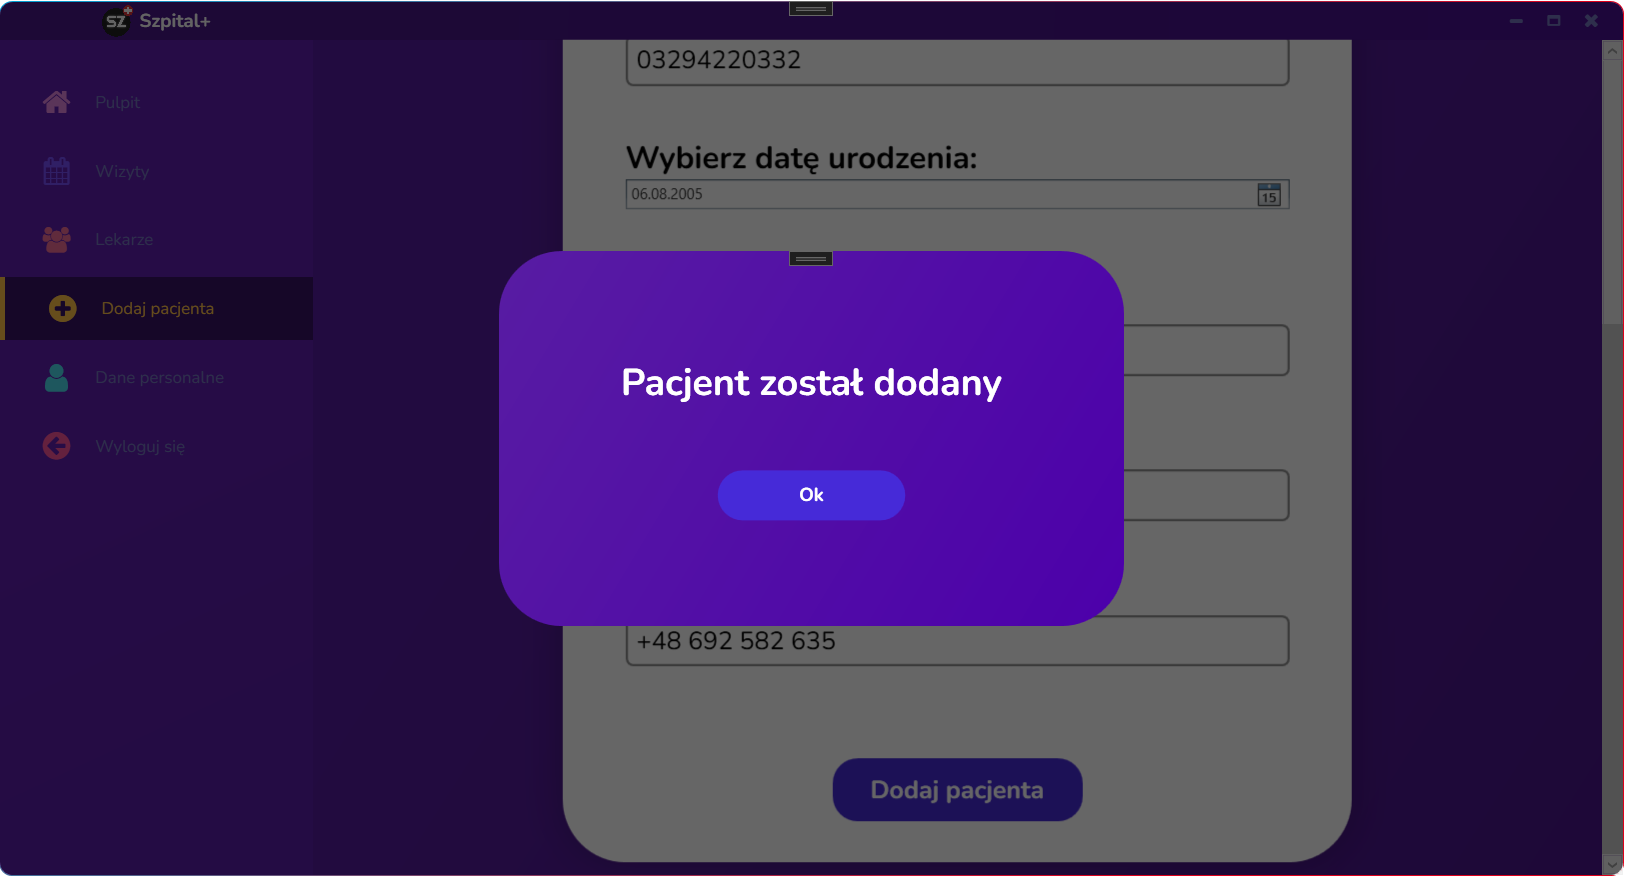
\includegraphics[height=6cm]{images/pacj_zost_dod.png}
        \caption{Pacjent został dodany}
        \label{fig:pacj_zost_dod}
	\end{center}
    \end{figure}
    \begin{figure}[H]
    \centering
    \subfigure{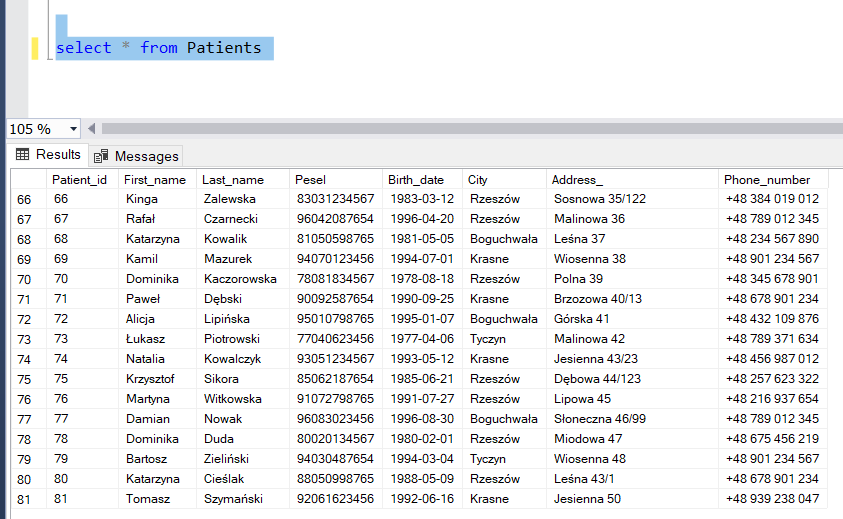
\includegraphics[width=0.6\textwidth]{images/pacjen_przed_dod.png}} 
    \subfigure{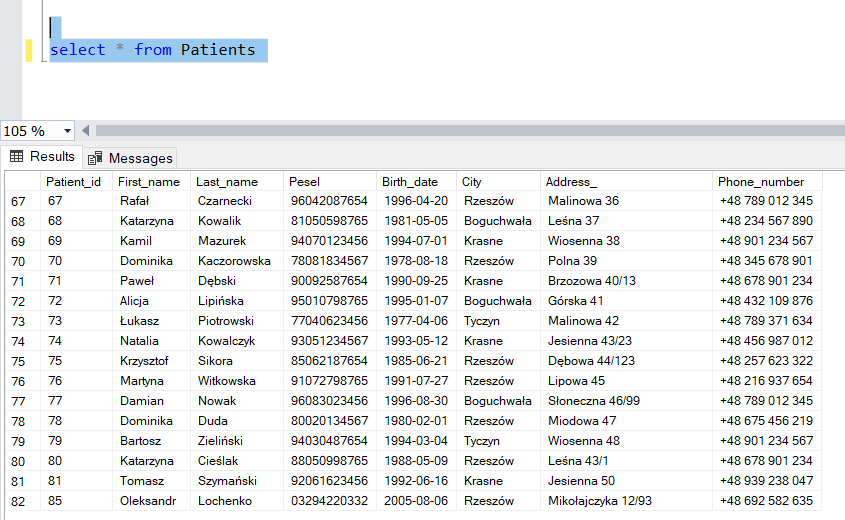
\includegraphics[width=0.6\textwidth]{images/pacjen_po_dod.png}}
    \caption{Tabela pacjentów przed i po dodaniu rekordu}
    \end{figure}

    \subsection{\Large{Okna dla głównego kierownika}}
    \subsubsection{\large{Pracownicy}}
    \begin{figure}[H]
        \begin{center}
	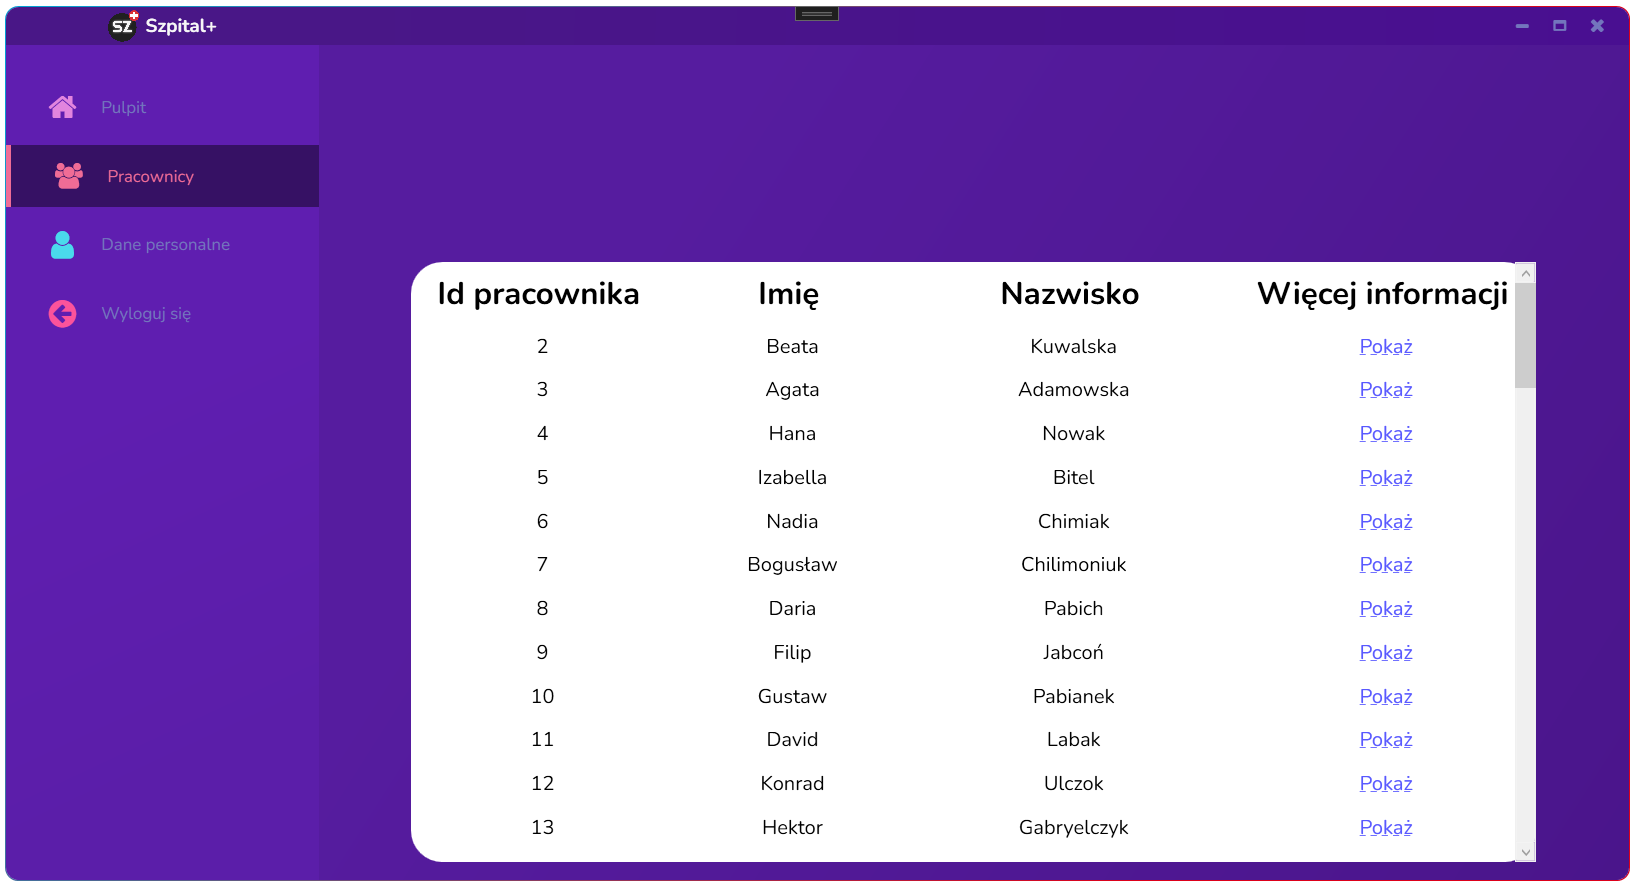
\includegraphics[height=7cm]{images/gl_kier_prac.png}
        \caption{Okno głównego kierownika(Pracownicy)}
        \label{fig:gl_kier_prac}
	\end{center}
    \end{figure}
    \hspace{5mm}Przycisk \textquotedbl Pokaż\textquotedbl{} nie został zaimplementowany.

    \subsection{\Large{Okna dla kierownika}}
    \subsubsection{\large{Lekarze}}
    \begin{figure}[H]
        \begin{center}
	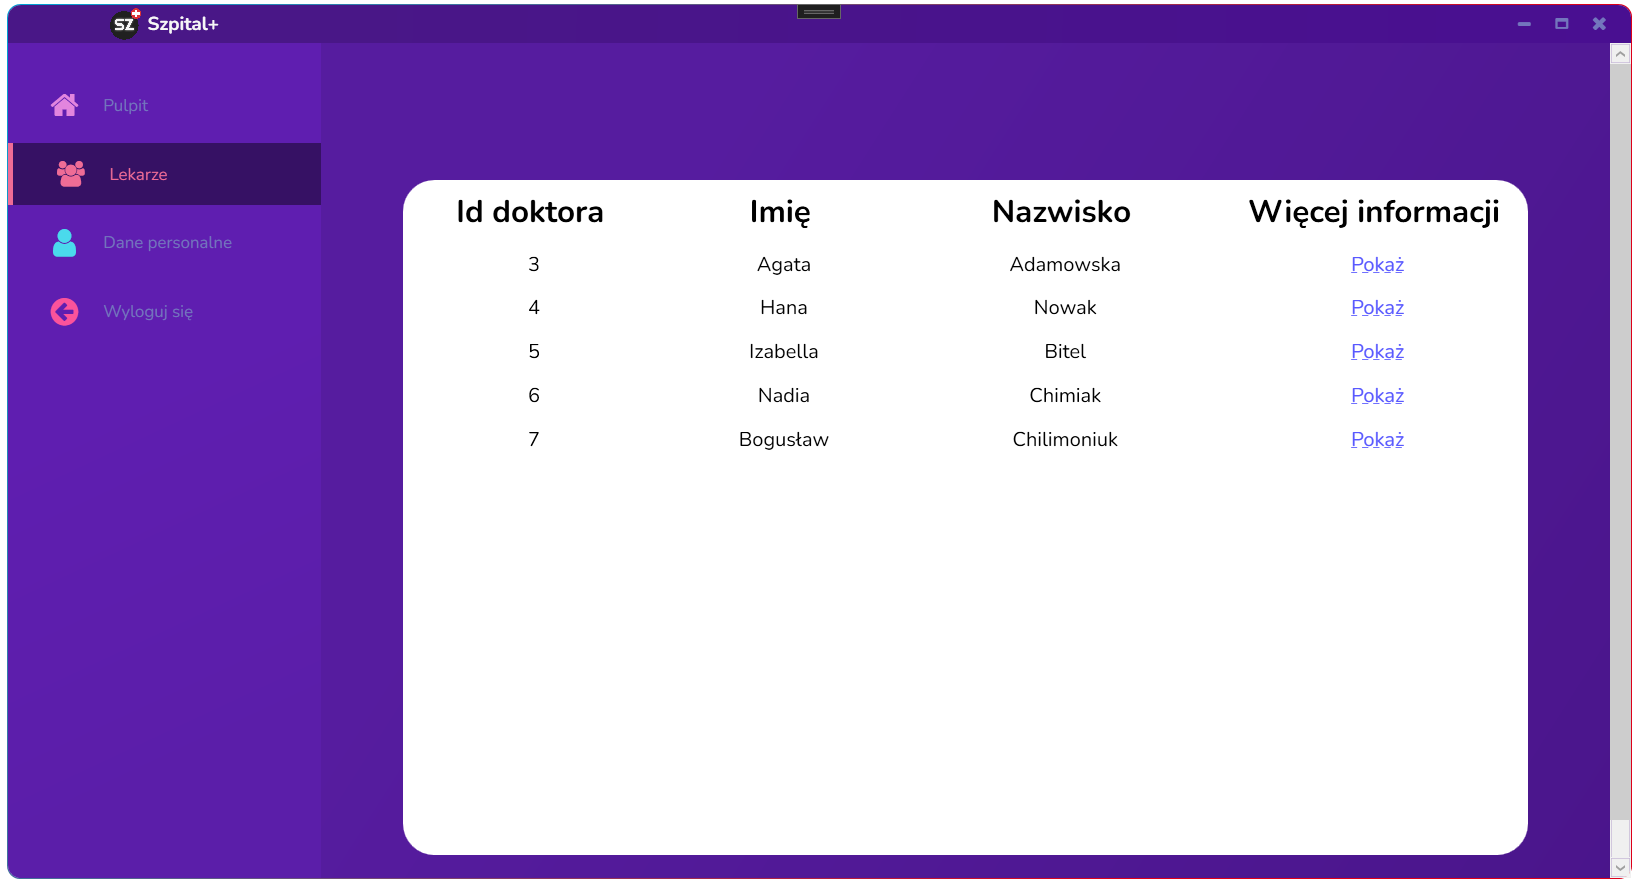
\includegraphics[height=7cm]{images/kier_lekar.png}
        \caption{Okno kierownika(Lekarze)}
        \label{fig:kier_lekar}
	\end{center}
    \end{figure}
    \hspace{5mm}Przycisk \textquotedbl Pokaż\textquotedbl{} nie został zaimplementowany.

    \subsection{\Large{Okna dla doktora}}
    \subsubsection{\large{Wizyty - nie został zaimplementowany}}
    
\end{flushleft}

% *************** Podsumowanie ***************
\begin{flushleft}
\section{\LARGE{Podsumowanie}}
\end{flushleft}

\begin{flushleft}
    \hspace{5mm}Podczas robienia projektu nauczyłem się planowania harmonogramu projektu(\ref{sec:harmon_proj}), implementacji wzoru MVVM(\ref{href:MVVM}), pisania interfejsu użytkownika(\ref{href:XAML}), pracy w środowisku Visual Studio(\ref{href:VStudio}) i programowania w języku C\#(\ref{href:c_sh}).
    \\
    \hspace{5mm}Dalsza praca będzie polegała na zrealizowaniu wszystkich funkcjonalności których nie zdążyłem zaimplementować, poprawienie i dopasowanie widoków, dodanie animacji oraz ulepszenie wydajności aplikacji.
\end{flushleft}


% *************** Literatura ***************
\newpage
\begin{flushleft}
\section{\LARGE{Literatura}}
\end{flushleft}

% *************** Bibliografia ***************
\begin{thebibliography}{6}
%dodanie wpisu do spisu bibliograficznego

\bibitem{www-1} https://www.youtube.com/watchv=oSeYvMEH7jc\&ab\_channel=tutorialsEU
\bibitem{www-2} https://www.youtube.com/watchv=oSeYvMEH7jc\&t=3533s\&ab\_channel=tutorialsEU
\bibitem{www-3}
https://www.youtube.com/watch?v=PzP8mw7JUzI\&t=1712s\&ab\_channel=Payload
\bibitem{www-4}
https://stackoverflow.com/questions/833943/watermark-hint-placeholder-text-in-textbox
\bibitem{www-5}
https://leanactionplan.pl/wykres-gantta/
\bibitem{www-6}
https://pl.wikipedia.org/wiki/Windows\_Presentation\_Foundation
\bibitem{www-7}
https://pl.wikipedia.org/wiki/.NET\_Framework
\bibitem{www-8}
https://pl.wikipedia.org/wiki/Extensible\_Application\_Markup\_Language
\bibitem{www-9}
https://en.wikipedia.org/wiki/Model\%E2\%80\%93view\%E2\%80\%93viewmodel
\bibitem{www-10}
https://stackoverflow.com/questions/58272836/display-datetime-in-textblock-with-dashed-underlined-textdecorations
\bibitem{www-11}
https://stackoverflow.com/questions/30231252/disable-main-window-wpf
\bibitem{www-12}
https://stackoverflow.com/questions/26258450/how-do-i-add-a-bullet-point-in-front-of-a-text-binding-in-wpf
\end{thebibliography}
\newpage

\newpage
%spis rysunków
\addcontentsline{toc}{chapter}{Spis rysunków}
\listoffigures
\newpage

\end{document}